\documentclass[11pt]{article}
\usepackage[utf8]{inputenc}
\usepackage{algorithm}
\usepackage{algorithmic}
\usepackage{amsfonts}
\usepackage{amsmath}
\usepackage{amssymb}
\usepackage{amsthm}
\usepackage[english]{babel}
\usepackage{booktabs}
\usepackage[labelfont=bf, font=small]{caption}
\usepackage{chngcntr}
\usepackage{color, colortbl}
\usepackage{fancyhdr}
\usepackage{graphicx}
\usepackage[utf8]{inputenc}
\usepackage{listings}
\usepackage{microtype}
\usepackage[numbers]{natbib}
\usepackage{parskip}
\usepackage{subcaption}
\usepackage[most]{tcolorbox}
\usepackage{xcolor}

\usepackage[vcentering,dvips]{geometry}
\geometry{
    papersize={7in,9in},
    bottom=3pc,
    top=5pc,
    left=5pc,
    right=5pc,
    bmargin=4.5pc,
    footskip=18pt,
    headsep=25pt}


\usepackage[
  colorlinks=true,
  linkcolor=black,
  anchorcolor=black,
  citecolor=black,
  filecolor=black,
  menucolor=black,
  runcolor=black,
  urlcolor=black]{hyperref}

\setcounter{tocdepth}{2}

\definecolor{Gray}{gray}{0.9}
\newcommand{\dotscale}{0.7}

\theoremstyle{definition}
\renewcommand\qedsymbol{$\blacksquare$}
\newtheorem{example}{Example}[section]

% Section numbers in captions.
\counterwithin{figure}{section}
\counterwithin{table}{section}
\counterwithin{example}{section}
\counterwithin{algorithm}{section}

\fancyhf{}
\lhead{\leftmark}
\rhead{\thepage}
\pagestyle{fancy}

%% log-sum-exp
\DeclareMathOperator*{\LSE}{\textrm{LSE}}

%% Matrices
\newcommand{\mA}{{\bf A}}
\newcommand{\mB}{{\bf B}}
\newcommand{\mC}{{\bf C}}
\newcommand{\mX}{{\bf X}}

%% Vectors
\newcommand{\va}{{\bf a}}
\newcommand{\vr}{{\bf r}}
\newcommand{\vu}{{\bf u}}
\newcommand{\vv}{{\bf v}}
\newcommand{\vx}{{\bf x}}
\newcommand{\vy}{{\bf y}}
\newcommand{\vz}{{\bf z}}

%% Graphs
\newcommand{\gA}{\mathcal{A}}
\newcommand{\gB}{\mathcal{B}}
\newcommand{\gC}{\mathcal{C}}
\newcommand{\gE}{\mathcal{E}}
\newcommand{\gG}{\mathcal{G}}
\newcommand{\gI}{\mathcal{I}}
\newcommand{\gN}{\mathcal{N}}
\newcommand{\gP}{\mathcal{P}}
\newcommand{\gT}{\mathcal{T}}
\newcommand{\gU}{\mathcal{U}}
\newcommand{\gX}{\mathcal{X}}
\newcommand{\gY}{\mathcal{Y}}
\newcommand{\gZ}{\mathcal{Z}}

%% Language
\renewcommand\L{\mathcal{L}}

%% <s>, </s>, and <b> tokens
\newcommand{\sos}{\textrm{\textless s\textgreater}}
\newcommand{\eos}{\textrm{\textless /s\textgreater}}
\newcommand{\blank}{\textrm{\textless b\textgreater}}


\title{An Introduction to Weighted Automata \\ in Machine Learning}
\author{Awni Hannun\footnote{
  Send correspondence to
  \href{mailto:awni.hannun@gmail.com}{awni.hannun@gmail.com}}}

\begin{document}

\maketitle

\begin{abstract}
    The goal of this work is to introduce the reader to weighted finite-state
    automata and their application to machine learning. I begin by motivating
    the use of automata in machine learning and proceed with an introduction to
    acceptors, transducers, and their associated properties. Many of the core
    operations of weighted automata are then described in detail. Following
    this, the work moves closer to the research frontier by explaining
    automatic differentiation and its use with weighted automata. The last
    section presents several extended examples to gain deeper familiarity with
    weighted automata, their operations, and their use in machine learning.
\end{abstract}

\tableofcontents

\section{Introduction}
\label{sec:introduction}

Finite-state automata have a relatively long history of application
in machine learning. The majority of these applications involve sequential
data.  For example, they are or have been used in speech recognition, machine
translation, protein function analysis, and other tasks in natural language
and computational biology.

However, the application of these data structures in machine learning is far
from main stream. In fact, their use decreased with the advent of end-to-end
deep learning. However, the recent development of frameworks for automatic
differentiation with automata suggests there may be renewed interest in the
application of automata to machine learning.

This tutorial introduces weighted automata and their operations. Once this
fundamental data structure is well understood, we then continue to build our
intuition by working through some extended examples. At minimum, I hope that
this tutorial engenders an appreciation for the potential of automata in
machine learning. Ideally for some readers this tutorial will be a launching
point for the incorporation of automata in machine-learning research and
applications.

However, before launching into the more technical content, let's start with
some broader perspectives in order to motivate the use of automata in machine
learning.

\subsection{Monolithic or Modular}

In the past, complex machine-learning systems, like those used in speech
recognition, involved many specialized hand-engineered components. The trend is
now towards the opposite end of the spectrum. Most machine-learning applications
involve a single, monolithic neural network. Both of these extremes have
advantages, and both have disadvantages.

A primary advantage of automata in machine learning is their ability to harness
the best of both worlds. Automata are capable of retaining many if not all of
the advantages of a multi-component, hand-engineered system as well as those of
a monolithic deep neural network. The next few paragraphs explain some of these
advantages and the regime to which they apply.

\paragraph{Modular:} One of the advantages of multi-component, hand-engineered
systems over monolithic neural networks is modularity. In traditional software
design modularity is a good thing. Modular systems are easier to develop since
part of the system can be changed without needing to change the rest. In
machine-learning systems, modularity is useful to avoid retraining the entire
system when only part of the model needs to be updated. Modularity can also be
useful when the individual modules can be reused. For example, speech
recognition systems are built from acoustic models and language models.
Acoustic models can be language agnostic and used for different languages.
Language models are general text based models which can be used in many
different tasks other than speech recognition.

\paragraph{Compound errors:} A primary disadvantage of modular systems is that
errors compound. Each module is typically developed in isolation and hence
unaware of the types of errors made by the modules from which it receives
input. Monolithic systems on the other hand can be thought of as being
constructed from many sub-components all of which are jointly optimized towards
a single objective. These sub-components can learn to compensate for the
mistakes made by the others and in general work together more cohesively.

\paragraph{Adaptable:} Modular systems are typically more adaptable than
monolithic systems. A machine-learning model which is tuned for one domain
usually won't work in another domain without retraining at least part of the
model on data from the new domain. Monolithic neural networks typically require
a lot of data and hence are difficult to adapt to new domains. Modular systems
also need to be adapted. However, in some cases only a small subset of the
modules need be updated. Adapting only a few sub-modules requires less data and
makes the adaptation problem simpler.

\paragraph{Learn from data:} One of the hallmarks of deep neural networks is
their ability to continue to learn and improve with larger data sets. Because
of the many assumptions hard-wired into more traditional modular systems, they
hit a performance ceiling much earlier as data set sizes increase. Retaining
the ability to learn when data is plentiful is a critical feature of any
machine-learning system.

\paragraph{Prior knowledge:} On the other hand, one of the downsides of deep
neural networks is their need for large data sets to yield even decent
performance. Encoding prior knowledge into a model improves sample efficiency
and hence reduces the need for data. Encoding prior knowledge into a deep
neural networks is not easy. In some cases, indirectly encoding prior knowledge into a
neural network can be done, such as the translation invariance implied by
convolution and pooling. However, in general, this is not so straightforward.
Modular systems by their very nature incorporate prior knowledge for a given
task. Each module is designed and built to solve a specific sub-task, usually
with plenty of potential for customization towards that task.

Modular and monolithic systems have complementary advantages with respect to
these four traits. Ideally we could construct machine-learning models which
retain the best of each. Automata-based models will take us a step closer
towards this goal. However, to use automata to their full potential we have to
overcome a couple of challenges. The key is enabling the use of weighted
automata in training the model itself. This requires 1) efficient
implementations and 2) easy to use frameworks which support automatic
differentiation.

\subsection{Advantages of Differentiable Automata}
\label{sec:advantages}

A key to unlocking the potential of automata in machine learning is enabling
their use during the training stage of machine-learning models. All of the
operations I introduce later are differentiable with respect to the arc weights
of their input graphs. This means that weighted automata and the operations on
them can be used in the same way that tensors and their corresponding
operations are used in deep learning. Operations can be composed to form complex
computation graphs. Some of the weighted automata which are input to the
computation graph can have parameters which are learned. These parameters can
be optimized towards an objective with gradient descent.

Automatic differentiation makes computing gradients for complex computation
graphs much simpler. Hence, combining automatic differentiation with weighted
automata is important to enabling their use in training machine-learning
models.

Sophisticated machine-learning systems often separate the training and
inference stages of the algorithm. Multiple models are trained in isolation via
one code path. For prediction on new data, the individual models are combined
and rely on a different code path. The constraints of the two regimes (training
and inference) are such that separation from a modeling and software
perspective is often the best option. However, this is not without drawbacks.

First, from a pragmatic standpoint, having separate logic and code paths for
training and inference requires extra effort and usually results in bugs from
subtle mismatches between the two paths. Second, from a modeling standpoint,
optimizing individual models in isolation and then combining them is
sub-optimal.

One of the benefits of combining automatic differentiation with weighted
automata is the potential to bring the training and inference stages closer
together. For example, speech recognition systems often use hand-implemented
loss functions at training time. However, the decoder (used for inference)
brings together multiple models represented as automata (lexicon, language model,
acoustic model, \emph{etc.}) in a completely different code path. By enabling
automatic differentiation with graphs, the decoding stage can also be used for
training. This has the potential to both simplify and improve the performance
of the system.

Combining automatic differentiation with automata creates a separation of code
from data. Loss functions like Connectionist Temporal Classification, the
Automatic Segmentation criterion, and Lattice-Free Maximum Mutual Information
have custom and highly optimized software implementations. However, these loss
functions can all be implemented using graphs and (differentiable) operations
on graphs. This separation of code from data, where graphs represent the data
and operations on graphs represent the code, has several benefits. First, the
separation simplifies the software. Second, the separation facilitates research
by making it easier to experiment with new ideas. Lastly, the separation
enables the optimization of graph operations to be more broadly shared.

\subsection{Comparison to Tensors}
\label{sec:comparison_to_tensors}

Modern deep learning is built upon the tensor data structure and the many
operations which take as input one or more tensors. Some of the more common
operations include matrix multiplication, two-dimensional convolution,
reduction operations (sum, max, product, \emph{etc}), and unary and binary
operations.

Automata are an alternative data structure and the operations are quite
different in general. However, one can draw a loose analogy between the categories
of operations with automata and those with tensors.
Table~\ref{tab:tensor_wfst_analogy} shows some of the common operations on
tensors and their analogous operations on automata. The analogy is quite loose,
but still useful at the very least as a mnemonic device and perhaps can help
build intuition for the various operations on graphs.

For example, superficially the formula for matrix multiplication and transducer
composition are quite similar. Assume we have three matrices such that $\mC = \mA
\mB$. The element at position $(i, j)$ of $\mC$ is given by:
\begin{equation}
    C_{ij} = \sum_{k} A_{ik} B_{kj}.
\end{equation}
Assume we have three transducers (graphs) where $\gC$ is the composition of
$\gA$ and $\gB$, then the score of the path pair $(\vu, \vv)$ is given by:
\begin{equation}
    \mathcal{C}(\vu, \vv) = \LSE_{\vr} \mathcal{A}(\vu, \vr) + \mathcal{B}(\vr, \vv),
\end{equation}
where $\LSE$ is the \emph{log-sum-exp} operation. Don't worry if the details
are not clear -- section~\ref{sec:advanced_operations} covers transducer
composition. The point is that both operations, transducer composition and
matrix multiplication, accumulate over an inner variable the values from each
of the inputs. In matrix multiplication this is the shared dimension of the
matrices $\mA$ and $\mB$. In graph composition the inner variable is the shared
path $\vr$.

\begin{table}[ht]
    \small
    \renewcommand{\arraystretch}{1.4}
    \caption{The table shows loosely analogous operations between tensors and
    automata (acceptors and transducers).}
    \centering
    \begin{tabular}{l l l}
    \toprule
        Tensor & Automata \\
    \midrule
        Matrix multiplication, convolution & Intersect, compose \\
        \rowcolor{Gray} Reduction ops (sum, max, prod, \emph{etc.}) & Shortest distance (forward, Viterbi) \\
        Unary ops (power, negation, \emph{etc.})  & Unary ops (closure) \\
        \rowcolor{Gray} $n$-ary ops (addition, subtraction, \emph{etc.})  & $n$-ary ops (concatenation, union) \\
    \bottomrule
    \end{tabular}
    \label{tab:tensor_wfst_analogy}
\end{table}

A higher-level analogy to tensor-based deep learning can also be made. Modern
machine-learning frameworks like PyTorch and TensorFlow (and their ancestors
like Torch and Theano) were critical to the success of tensor-based deep
learning. These frameworks include support for automatic differentiation. They
also provide easy to use access to extremely efficient implementations of the
core operations. In the same way, automata-based machine learning should
benefit from frameworks with these features. We are just beginning to see new
developments in frameworks for automata-based machine learning including
GTN\footnote{I am a co-author of the GTN framework which is open source at
\url{https://github.com/gtn-org/gtn}} and k2.\footnote{The k2 framework is the
successor of Kaldi and is open source at \url{https://github.com/k2-fsa/k2}}
Perhaps these will encourage the use of automata in machine learning.

\subsection{History and Bibliographic Notes}

\citet{hopcroft2001introduction} provides an excellent introduction to
non-weighted automata. \citet{mohri2009weighted} gives a more formal and
general treatment of weighted automata and associated algorithms.

Weighted finite-state automata are commonly used in speech recognition, natural
language processing, optical character recognition, and other
applications~\citep{breuel2008ocropus, knight2009applications, mohri1997finite,
mohri2002weighted, mohri2008speech}. \citet{pereira1997} developed an early
application of weighted automata to speech recognition, though before that
there were other applications in natural language
processing~\citep{pereira1994weighted, sproat1996stochastic}. The Graph
Transformer Networks of~\citet{bottou97}, a similar though more general
framework, were developed around the same time and applied to character
recognition in images.

The sequence criteria mentioned in section~\ref{sec:advantages}, namely
Connectionist Temporal Classification~\citep{graves2006}, the Automatic
Segmentation criterion~\citep{collobert2016wav2letter}, and Lattice-free
Maximum Mutual Information~\citep{povey2016purely}, are most commonly used in
speech recognition. Section~\ref{sec:extended_examples} shows how to implement
a subset of these using weighted automata. \citet{hannun2017sequence} gives a
more detailed introduction to Connectionist Temporal Classification.

In terms of software, two of the better known libraries for operations on WFSTs
are OpenFST~\citep{allauzen2007openfst} and its predecessor
FSM~\citep{mohri2000design}. In section~\ref{sec:comparison_to_tensors}, I
compared weighted automata to tensors. PyTorch~\citep{paszke2019pytorch} and
TensorFlow~\citep{abadi2016tensorflow} are two of the most used libraries for
tensor-based deep learning with automatic differentiation. These were based on
earlier frameworks including Torch~\citep{collobert2011torch7} and
Theano~\citep{bergstra2010theano}. Libraries which support automatic
differentiation with weighted automata have only recently been
developed~\citep{k2, hannun2020differentiable}.

\section{Acceptors and Transducers}
\label{sec:acceptors_transducers}

\subsection{Automata}
\label{sec:automata}

The broad class of graphs we are going to look at are finite-state automata.
These include deterministic finite-state automata (DFAs) and non-deterministic
finite-state automata (NFAs). More specifically we will consider a
generalization of DFAs and NFAs called weighted finite-state acceptors (WFSAs).
That's a mouthful, so I will just call them \emph{acceptors}. We will also
consider a further generalization of an acceptor called a \emph{transducer}
(weighted finite-state transducers or WFSTs). Figure~\ref{fig:wfsa_classes}
shows the relation between these three graphs; transducers, acceptors, and
automata. Transducers are the most expressive in terms of their
representational power, followed by acceptors followed by unweighted automata.

\begin{figure}
    \centering
    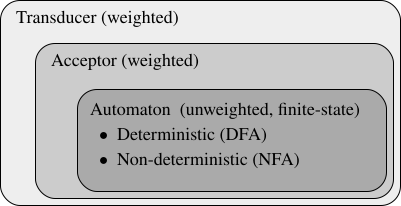
\includegraphics[width=0.7\linewidth]{figures/wfsa_classes}
    \caption{A hierarchy of automata classes from general to specific in terms
    of representation power. Weighted transducers can represent anything that
    weighted acceptors can represent. Weighted acceptors in turn can represent
    any unweighted finite-state automata.}
    \label{fig:wfsa_classes}
\end{figure}

Before we dive into acceptors and transducers, let's introduce some general
graph terminology that I will use throughout. In the following graph a
\emph{state} or \emph{node} is represented by a circle. The arrows represent
connections between two states. We usually refer to these as \emph{arcs} but
sometimes also \emph{edges}. The graph is directed since the connections
between states are unidirectional arrows. The arcs in a graph can have labels.
In figure~\ref{fig:simple_automata} the arc between states $0$ and $1$ has a
label of $a$. Similarly, the arc between states $1$ and $2$ has a label of $b$.
The graph is an example of a finite-state automata (FSA) or finite-state
machine (FSM), so called because it has a finite number of nodes.

\begin{figure}
    \centering
    \includegraphics{figures/simple_automata}
    \caption{An example of a simple finite-state automata.}
    \label{fig:simple_automata}
 \end{figure}

An automata is deterministic if for each state and label pair there is only one
outgoing transition which matches that label. An automata is nondeterministic
if multiple transitions leaving a state have the same label. The graphs in
figure~\ref{fig:dfa_nfa} show an example of a deterministic and a
nondeterministic automata. In general, acceptors and transducers to can be
nondeterministic.

\begin{figure}
    \centering
    \begin{subfigure}[b]{0.48\textwidth}
        \includegraphics[scale=\dotscale]{figures/simple_dfa}
        \caption{Deterministic}
        \label{fig:simple_dfa}
    \end{subfigure}
    \begin{subfigure}[b]{0.48\textwidth}
        \includegraphics[scale=\dotscale]{figures/simple_nfa}
        \caption{Nondeterministic}
        \label{fig:simple_nfa}
    \end{subfigure}
    \caption{An example of a deterministic automata and a nondeterministic
    automata. The nondeterministic automata has two arcs leaving state $0$ both
    with label $a$ and two arcs leaving state $2$ both with the label $c$.}
    \label{fig:dfa_nfa}
\end{figure}

\subsection{Acceptors}

Let's start by constructing some very basic automata to get a feel for their
various properties.

The start state $s = 0$ has a bold circle around it. The accepting state $1$ is
represented with concentric circles. Each arc has a label and a corresponding
weight. So the first arc from state $0$ to state $1$ with the text $a/0$ means
the label is $a$ and the weight is $0$. The fact that there is only a single
label on each arc means this graph is an \emph{acceptor}. Since it has weights,
we say its a weighted acceptor. Since the number of states is finite, some
would call it a weighted finite-state acceptor or WFSA. Again, that's a
mouthful, so I'll just call these graphs acceptors.

\begin{figure}
    \centering
    \includegraphics[scale=\dotscale]{figures/simple_fsa}
    \caption{An example of a simple acceptor. The label on each arc shows the
    input label and weight, so the $a/0$ represents a label of $a$ and a weight
    of $0$.}
    \label{fig:simple_fsa}
\end{figure}

An accepting path in the graph is a sequence of arcs which begin at a start
state and end in an accepting state. By concatenating the labels on an
accepting path, we get a string which is accepted by the graph. So the string
$aa$ is accepted by the graph by following the state sequence $0 \rightarrow 2
\rightarrow 1$. The string $ba$ is also accepted by the graph by following the
same state sequence but taking the arc with label $b$ when traversing from
state $0$ to state $1$. The language of the acceptor is the set of all strings
which are accepted by it. You may also encounter ``recognized'' used as a
synonym for ``accepted''. Let the variable $\gA$ represent the acceptor in
figure~\ref{fig:simple_fsa}. In general, I'll use uppercase script letters to
represent graphs. Let $\mathcal{L}(\gA)$ denote the language of $\gA$. In this
case $\mathcal{L}(\gA) = \{aa, ba\}$.

There are different ways to compute the weight of a string accepted by the
graph. The most common is to sum the weights of the arcs on the accepting path
for that string. For example the string $aa$ in the graph in
figure~\ref{fig:simple_fsa} has a weight of $0 + 2 = 2$. Another option would
be to multiply the weights. These two options correspond to interpreting the
weights as either log probabilities or probabilities. We'll have more to say
about this later.

The graph in figure~\ref{fig:multi_path} accepts the same sequence by multiple
paths.

\begin{figure}
    \centering
    \includegraphics[scale=\dotscale]{figures/multi_path}
    \caption{An acceptor which has multiple paths for the same sequence, $aa$.}
    \label{fig:multi_path}
\end{figure}

The string $aa$ is accepted along the state sequence $0 \rightarrow 2
\rightarrow 1$ and along the state sequence $0 \rightarrow 3 \rightarrow 1$. In
this case, to compute the score of $aa$ we need to consider both paths. Again
we have a couple of options here. The most common approach is to
\emph{log-sum-exp} the individual path scores. Again this corresponds to
interpreting the path scores as log probabilities. We'll use $\LSE(s_1, s_2)$
to denote the \emph{log-sum-exp} of the two scores $s_1$ and $s_2$:
\begin{equation}
\LSE(s_1, s_2) = \log \left( e^{s_1} + e^{s_2}\right).
\end{equation}
So the overall weight for the string $aa$ in the graph in
figure~\ref{fig:multi_path} is given by:
$$
\log \left(e^{0 + 2} + e^{1 + 3}\right) = 4.13.
$$

Acceptors can have multiple start states and multiple accept states. In the
graph in figure~\ref{fig:multi_start_accept}, the states $0$ and $1$ are both
start states, and the states $3$ and $4$ are both accept states.

\begin{figure}
    \centering
    \includegraphics[scale=\dotscale]{figures/multi_start_accept}
    \caption{An acceptor with multiple start states ($0$ and $1$) and multiple
    accept states ($3$ and $4$).}
    \label{fig:multi_start_accept}
\end{figure}

It turns out that allowing multiple start or accept states does not increase
the expressive power of the graph. With $\epsilon$ transitions (which we will
discuss soon), one can convert any graph with multiple start states and
multiple accept states into an equivalent graph with a single start state and a
single accept state.

Note also that start states can have incoming arcs (as in state $1$) and accept
states can have outgoing arcs, as in state $3$.

\begin{example}
Compute the score of the string $ab$ in figure~\ref{fig:multi_start_accept}.
\end{example}

\begin{proof}[\unskip\nopunct]
The two state sequences which accept the string $ab$ are the states $0
\rightarrow 2 \rightarrow 3$ and $1 \rightarrow 3 \rightarrow 4$. The overall
score is given by:
$$
\log (e^{1 + 3} + e^{1 + 2}) = 4.31.
$$
\end{proof}

Graphs can also have self-loops and cycles. For example, the graph in
figure~\ref{fig:fsa_loops} has a self-loop on the state $0$ and a cycle
following the state sequence $0 \rightarrow 1 \rightarrow 2 \rightarrow 0$.

\begin{figure}
    \centering
    \includegraphics[scale=\dotscale]{figures/fsa_loops}
    \caption{A graph with a self-loop on the state $0$ and a cycle from $0
    \rightarrow 1 \rightarrow 2 \rightarrow 0$.}
    \label{fig:fsa_loops}
\end{figure}

The language of a graph with cycles and self-loops contains infinitely many
strings.  For example, the language of the graph in figure~\ref{fig:fsa_loops}
includes any string that starts with zero or more $a$s and ends in $bb$. As a
regular expression we write this as $a^*bb$ where the $^*$ denotes zero or more
$a$s.

The $\epsilon$ symbols has a special meaning when it is the label on an arc.
Any arc with an $\epsilon$ label can be traversed without consuming an input
token in the string. So the graph in figure~\ref{fig:fsa_epsilon} accepts the
string $ab$, but it also accepts the string $b$ because we can traverse from
state $0$ to state $1$ without consuming an input.

\begin{figure}
    \centering
    \includegraphics[scale=\dotscale]{figures/fsa_epsilon}
    \caption{An acceptor with an $\epsilon$ transition on the second arc
    between state $0$ and $1$.}
    \label{fig:fsa_epsilon}
\end{figure}

As it turns out, any graph with $\epsilon$-transitions can be converted to an
equivalent graph without $\epsilon$ transitions. However, this usually comes at
a large cost in the size of the graph. Complex languages can be represented by
much more compact graphs with the use of $\epsilon$-transitions.

\begin{example}
Convert the graph in figure~\ref{fig:multi_start_accept} which has multiple
start and accept states to an equivalent graph with only a single start and
accept state using $\epsilon$ transitions.
\end{example}

\begin{proof}[\unskip\nopunct]
The graph in figure~\ref{fig:epsilon_start_accept} is the equivalent graph
with a single start state and a single accept state.

\begin{figure}
    \centering
    \includegraphics[scale=\dotscale]{figures/epsilon_start_accept}
    \caption{The equivalent graph using only a single start state and accept
    state to the graph in figure~\ref{fig:multi_start_accept} which has
    multiple start and accept states.}
    \label{fig:epsilon_start_accept}
\end{figure}

The construction works by creating a new start state and connecting it to the
old start states with $\epsilon$ transitions with a weight of $0$. The old
start nodes are regular internal nodes in this new graph. Similarly the old
accept states are now regular states and they connect to the new accept state
with $\epsilon$ transitions with a weight of $0$.
\end{proof}

\subsection{Transducers}

A \emph{transducer} maps input strings to output strings. Transducers are a
generalization of acceptors. Every acceptor is a transducer, but not every
transducer is an acceptor. Let's look at a few example transducers to
understand how they work.

The arc labels distinguish an acceptor from a transducer. A transducer has both
an input and output arc label. The arc labels are of the form $a\!:\!x/0$ where
$a$ is the input label $x$ is the output label and $0$ is the weight. An
acceptor can be represented as a transducer where the input and output labels
on every arc are identical.

\begin{figure}
    \centering
    \includegraphics[scale=\dotscale]{figures/simple_fst}
    \caption{An example of a simple transducer. The label on each arc shows the
    input label, the output label, and the weight. So $a\!:\!x/0$ represents an
    input label of $a$, and output label of $x$, and a weight of $0$.}
    \label{fig:simple_fst}
\end{figure}

Instead of saying that a transducer accepts a given string, we say that it
\emph{transduces} one string to another. The graph in
figure~\ref{fig:simple_fst} transduces the string $ab$ to the string $xz$ and
the string $bb$ to the string $yz$. The weight of a transduced pair is
computed in the same way as in an acceptor. The scores of the individual arcs
on the path are summed. The path scores are combined with \emph{log-sum-exp}.
So the weight of the transduced pair $(ab, xz)$ in the graph in
figure~\ref{fig:simple_fst} is $0+3 = 3$.

We have to generalize concept of the language from an acceptor to a transducer.
I'll call this generalization the transduced set. Since it will always be clear
from context if the graph is an acceptor or transducer, I'll use the same
symbol $\mathcal{L}$ to represent the transduced set. If $\gT$ is a transducer,
then $\mathcal{L}(\gT)$ is the set of pairs of strings transduced by $\gT$.
More formally, a pair of strings $(\vx, \vy) \in \mathcal{L}(\gT)$ if $\gT$
transduces $\vx$ to $\vy$.

\begin{example}
Compute the score of the transduced pair $(aab, zyy)$ in the graph in
figure~\ref{fig:fst_example_score}.
\end{example}

\begin{proof}[\unskip\nopunct]
\begin{figure}
    \centering
    \includegraphics[scale=\dotscale]{figures/fst_example_score}
    \caption{An example transducer in which the sequence $aab$ is transduced to
    the sequence $zyy$ on multiple paths.}
    \label{fig:fst_example_score}
\end{figure}

The two paths which transduce $aab$ to $zyy$ are following the state sequence
$0 \rightarrow 1 \rightarrow 3 \rightarrow 3$ and $0 \rightarrow 0 \rightarrow
2 \rightarrow 3$. The score of the first path is $6$ and the score of the
second path is $6$. So the overall score is:
$$
\log \left(e^6 + e^6\right) = 6.69.
$$
\end{proof}

Transducers can also have $\epsilon$ transitions. The $\epsilon$ can be either
the input label on an arc, the output label on an arc, or both. When the
$\epsilon$ is the input label on an arc, it means we can traverse that arc
without consuming an input token, but we still output the arc's corresponding
output label. When the $\epsilon$ is the output label, the opposite is true.
The input is consumed but no output is produced. And when the $\epsilon$ is
both the input and the output label, the arc can be traversed without consuming
an input or producing an output.

\begin{figure}
    \centering
    \includegraphics[scale=\dotscale]{figures/fst_epsilon}
    \caption{A transducer with $\epsilon$ transitions. The $\epsilon$ can be
    just the input label, just the output label, or both the input and output
    label.}
    \label{fig:fst_epsilon}
\end{figure}

In the graph in figure~\ref{fig:fst_epsilon}, the string $b$ gets transduced to
the string $x$. On the first arc between states $0$ and $1$, we output an $x$
without consuming any token. On the second arc between states $1$ and $2$, a
$b$ is consumed without outputting any new token. Finally, on the arc between
states $2$ and $3$ we neither consume nor output a token.

\section{Basic Operations}
\label{sec:basic_operations}

An operation on a transducer (or acceptor) takes one or more transducers as
input and outputs a transducer. You can think of these operations as functions
on graphs. As a reminder, I'll use uppercase script letters to represent
graphs, so $\gA$ for example can represent a graph. Functions will be denoted
by lower case variables. So $f(\gA)$ is a function which takes as input a
single graph and outputs a graph.

\subsection{Closure}

The closure, sometimes called the Kleene star, is a unary function (takes a
single input) which can operate on either an acceptor or transducer. If the
sequence $\vx$ is accepted by $\gA$, then zero or more copies of $\vx$ are
accepted by the closure of $\gA$. More formally, if the language of an acceptor
is $\L(\gA)$, then the language of the closure of $\gA$ is $\{\vx^n
\mid \vx \in \L(\gA),\;\; n = 0, 1, \ldots, \}$. The notation $\vx^n$
means $\vx$ concatenated $n$ times. So $\vx^2$ is $\vx \vx$ and $\vx^0$ is the
empty string. Usually the closure of an acceptor is denoted by $^*$, as in
$\gA^*$. This is the same notation used in regular expressions.

The closure of a graph is easy to construct with the use of $\epsilon$
transitions. The language of the graph in figure~\ref{fig:fsa_pre_closure} is
the string $aba$.

\begin{figure}
    \centering
    \includegraphics[scale=\dotscale]{figures/fsa_pre_closure}
    \caption{An example of a simple acceptor with language $\{aba\}$, in other
    words $\L(\gA) = \{aba\}$.}
    \label{fig:fsa_pre_closure}
\end{figure}

The closure of the graph needs to accept an arbitrary number of copies of $aba$
including the empty string. To accept the empty string we make the start state
an accept state as well. To accept one or more copies of $aba$ we simply wire
up the old accept states to the new start state with $\epsilon$ transitions.

The closure of the graph in figure~\ref{fig:fsa_pre_closure} is shown in
figure~\ref{fig:fsa_closure}.

\begin{figure}
    \centering
    \includegraphics[scale=\dotscale]{figures/fsa_closure}
    \caption{The closure $\gA^*$ of the graph in
    figure~\ref{fig:fsa_pre_closure}. The language of the graph is $\{\epsilon,
    aba, abaaba, \ldots\}$.}
    \label{fig:fsa_closure}
\end{figure}

\begin{example}
You might notice that state $4$ in the graph in figure~\ref{fig:fsa_closure} is
not necessary. Consider an alternate construction for computing the
closure of a graph. We could have made the state $0$ into an accept state
and connected state $3$ to state $0$ with an $\epsilon$ transition, as in
the graph in figure~\ref{fig:fsa_closure_2}.

\begin{figure}
    \centering
    \includegraphics[scale=\dotscale]{figures/fsa_closure_2}
    \caption{The closure $\gA^*$ of the graph in
    figure~\ref{fig:fsa_pre_closure} using an alternate, simpler construction
    which connects the accept state to the original start state with an
    $\epsilon$ transition. This construction does not work for every case.}
    \label{fig:fsa_closure_2}
\end{figure}

For the graph in figure~\ref{fig:fsa_pre_closure}, this alternate construction
works and requires fewer states and arcs. In the general case, this
construction turns every start state into an accept state instead of adding
a new start state. Give an example where this doesn't work? In other words,
give an example where the graph from this modified construction is not the
correct closure of the original graph.
\end{example}

\begin{proof}[\unskip\nopunct]
An example for which the alternate construction does not work is shown in the
graph in figure~\ref{fig:fsa_pre_closure_wrong}. The language of the graph
is $a^nb$ (any number of $a$'s followed by a $b$) and the closure is
$(a^nb)^*$, or any sequence that ends with $b$.

\begin{figure}
    \centering
    \includegraphics[scale=\dotscale]{figures/fsa_pre_closure_wrong}
    \caption{An acceptor for which the alternate construction for the closure
    does not yield the correct result.}
    \label{fig:fsa_pre_closure_wrong}
\end{figure}

If we follow the modified construction for the closure, as in the graph in
figure~\ref{fig:fsa_closure_wrong}, then the language would incorrectly
include sequences that do not end with $b$ such as $a^*$. The graph
following the correct construction of the closure is in
figure~\ref{fig:fsa_closure_right}.

\begin{figure}
    \centering
    \includegraphics[scale=\dotscale]{figures/fsa_closure_wrong}
    \caption{The alternate construction which incorrectly computes the closure
    of the graph in figure~\ref{fig:fsa_pre_closure_wrong}.}
    \label{fig:fsa_closure_wrong}
\end{figure}


\begin{figure}
    \centering
    \includegraphics[scale=\dotscale]{figures/fsa_closure_right}
    \caption{The correct closure of the graph in
    figure~\ref{fig:fsa_pre_closure_wrong} which has the language $(a^nb)^*$, which
    is any sequence which ends with $b$.}
    \label{fig:fsa_closure_right}
\end{figure}

\end{proof}

\subsection{Union}

The union takes as input two or more graphs and produces a new graph. The
language of the resultant graph is the union of the languages of the input
graphs. More formally let $\gA_1, \ldots, \gA_n$ be $n$ graphs. The language of
the union graph is given by $\{ x \mid x \in \gA_i \textrm{ for some } i = 1,
\ldots, n \}$. I'll occasionally use the $+$ sign to denote the union, as in
$\gU = \gA_1 + \gA_2$.

Since we let a graph have multiple start states and multiple accept states, the
union is  easy to construct. A state in the union graph is a start state if it
was a start state in one of the original graphs. A state in the union graph is
an accept state if it was an accept state in one of the original graphs.

Consider the three graphs in figure~\ref{fig:union_inputs} with languages
$\{ab, aba, abaa, \ldots\}$, $\{ba\}$, and $\{ac\}$ respectively.

\begin{figure}
    \centering
    \begin{subfigure}[b]{0.8\textwidth}
        \centering
        \includegraphics[scale=\dotscale]{figures/union_1}
        \caption{}
    \end{subfigure}
    \par\bigskip
    \begin{subfigure}[b]{0.8\textwidth}
        \centering
        \includegraphics[scale=\dotscale]{figures/union_2}
        \caption{}
    \end{subfigure}
    \par\bigskip
    \begin{subfigure}[b]{0.8\textwidth}
        \centering
        \includegraphics[scale=\dotscale]{figures/union_3}
        \caption{}
    \end{subfigure}
    \caption{Three acceptors with languages $\{ab, aba, abaa, \ldots\}$,
    $\{ba\}$, and $\{ac\}$ from top to bottom, respectively.}
    \label{fig:union_inputs}
\end{figure}

Notice in the union graph in figure~\ref{fig:union} the only visual distinction
from the individual graphs is that the states are numbered consecutively from
$0$ to $8$ indicating a single graph with nine states instead of three
individual graphs. The language of the union graph is $\{ab, aba, abaa,
\ldots\} \cup \{ba\} \cup \{ac\}$.

\begin{figure}
    \centering
    \includegraphics[scale=\dotscale]{figures/union}
    \caption{The union of the three acceptors in figure~\ref{fig:union_inputs}
    with language $\{ab, aba, abaa, \ldots\} \cup \{ba\} \cup \{ac\}$.}
    \label{fig:union}
\end{figure}

\subsection{Concatenate}

Like union, concatenate produces a new graph given two or more graphs as
input. The language of the concatenated graph is the set of strings which can
be formed by any concatenation of strings from the individual graph.
Concatenate is not commutative, the order of the input graphs matters. More
formally the language of the concatenated graph is given by $\{\vx_1 \ldots
\vx_n \mid \vx_1 \in \L(\gA_1), \ldots, \vx_n \in \L(\gA_n)\}$. Occasionally, I
will denote concatenation by placing the graphs side-by-side. So $\gA_1 \gA_2$
represents the concatenation of $\gA_1$ and $\gA_2$.

The concatenated graph can be constructed from the original input graphs by
connecting the accept states of one graph to the start states of the next.
Assume we are concatenating $\gA_1, \ldots, \gA_n$. The start states of the
concatenated graph are the start states of the first graph, $\gA_1$. The accept
states of the concatenated graph are the accept states of the last graph,
$\gA_n$. For any two graph $\gA_i$ and $\gA_{i+1}$, we connect each accept
state of $\gA_i$ to each start state of $\gA_{i+1}$ with an $\epsilon$
transition.

\begin{figure}
    \centering
    \begin{subfigure}[b]{0.48\textwidth}
        \centering
        \includegraphics[scale=\dotscale]{figures/concat_1}
    \end{subfigure}
    \begin{subfigure}[b]{0.48\textwidth}
        \centering
        \includegraphics[scale=\dotscale]{figures/concat_2}
    \end{subfigure}
    \caption{The acceptor on left has language $\{ba\}$ and the acceptor on the
    right has language $\{ac, bc\}$.}
    \label{fig:concat_inputs}
\end{figure}

As an example, consider the two graphs in figure~\ref{fig:concat_inputs}. The
concatenated graph is in figure~\ref{fig:concat} and has the language $\{baac,
babc\}$.

\begin{figure}
    \centering
    \includegraphics[scale=\dotscale]{figures/concat}
    \caption{The graph is the concatenation of the two graphs in
    figure~\ref{fig:concat_inputs} and has the language $\{baac, babc\}$.}
    \label{fig:concat}
\end{figure}

\begin{example}
What is the identity graph for the concatenation function? The identity in a
binary operation is the value which when used in the operation leaves the second
input unchanged. In multiplication this would be $1$ since $c * 1 = c$ for any
real value $c$.

What is the equivalent of the annihilator graph in the concatenation function?
The annihilator in a binary operation is the value such that the operation with
the annihilator always returns the annihilator. For multiplication $0$ is the
annihilator since $c *0 = 0$ for any real value $c$.
\end{example}

\begin{proof}[\unskip\nopunct]
The graph which accepts the empty string is the identity. The graph which does
not accept any strings is the annihilator. See the
figure~\ref{fig:concat_identity_annihilator} for an example of these two
graphs.

\begin{figure}
    \centering
    \begin{subfigure}[b]{0.48\textwidth}
        \centering
        \includegraphics[scale=\dotscale]{figures/concat_identity}
        \caption{Identity}
        \label{fig:concat_identity}
    \end{subfigure}
    \begin{subfigure}[b]{0.48\textwidth}
        \centering
        \includegraphics[scale=\dotscale]{figures/concat_annihilator}
        \caption{Annihilator}
        \label{fig:concat_annihilator}
    \end{subfigure}
    \caption{The identity and the annihilator for the concatenate operation.
    The language of the identity graph is the empty string $\{\epsilon\}$. The
    language of the annihilator graph is the empty set $\{\}$.}
    \label{fig:concat_identity_annihilator}
\end{figure}

The identity graph is a single node which is both a start and accept state. The
language of the identity graph is the empty string. The annihilator graph is a
single non accepting state. The language of the annihilator graph is the empty
set. Note the subtle distinction between the language that contains the empty
string and the language that is the empty set. The former can be written as
$\{\epsilon\}$ whereas the latter is $\{\}$ (also commonly denoted by
$\varnothing$).
\end{proof}

\begin{example}
Construct the concatenation of the two graphs in
figure~\ref{fig:concat_example_inputs}.
\end{example}

\begin{proof}[\unskip\nopunct]

\begin{figure}
    \centering
    \begin{subfigure}[b]{0.48\textwidth}
        \centering
        \includegraphics[scale=\dotscale]{figures/concat_example_1}
    \end{subfigure}
    \begin{subfigure}[b]{0.48\textwidth}
        \centering
        \includegraphics[scale=\dotscale]{figures/concat_example_2}
    \end{subfigure}
    \caption{The acceptor on the left has the language $\{ba, bc\}$, the
    acceptor on the right has the language $\{a, c\}$.}
    \label{fig:concat_example_inputs}
\end{figure}

The concatenated graph is in figure~\ref{fig:concat_example}.

\begin{figure}
    \centering
    \includegraphics[scale=\dotscale]{figures/concat_example}
    \caption{The concatenation of the two graphs in
    figure~\ref{fig:concat_example_inputs} has the language $\{baa, bac, bca,
    bcc\}$.}
    \label{fig:concat_example}
\end{figure}

\end{proof}

\begin{example}
Suppose we have a list of graphs to concatenate $\gA_1, \ldots, \gA_n$ where the
$i$-th graph has $s_i$ start states and $a_i$ accept states. How many new
arcs will the concatenated graph require?
\end{example}

\begin{proof}[\unskip\nopunct]
For each consecutive pair of graphs $\gA_i$ and $\gA_{i+1}$, we need to add
$a_i * s_{i+1}$ connecting arcs in the concatenated graph. So the total
number of additional arcs is:
$$
\sum_{i=1}^{n-1} a_i * s_{i+1}.
$$
\end{proof}

\subsection{Summary}

We've seen three basic operations so far:

\begin{itemize}
    \item {\bf Closure:} The closed graph accepts any string in the input graph
        repeated zero or more times. The closure of a graph $\gA$ is denoted
        $\gA^*$.

    \item {\bf Union:} The union graph accepts any string from any of the input
        graphs. The union of two graphs $\gA_1$ and $\gA_2$ is denoted $\gA_1 +
        \gA_2$.

    \item {\bf Concatenate:} The concatenated graph accepts any string which
        can be formed by concatenating strings (respecting order) from the
        input graphs. The concatenation of two graphs $\gA_1$ and $\gA_2$ is
        denoted $\gA_1\gA_2$.

\end{itemize}

\begin{example}
Assume you are given the following individual graphs $\gA_a$, $\gA_b$, and
$\gA_c$, which recognize $a$, $b$, and $c$ respectively, as in
figure~\ref{fig:fsa_tokens}. Using only closure, union, and concatenate,
construct the graph which recognizes any number of repeats of the strings
$aa$, $bb$, and $cc$. For example $aabb$ and $bbaacc$ are in the language
but $b$ and $ccaab$ are not.
\end{example}

\begin{proof}[\unskip\nopunct]

\begin{figure}
    \centering
    \begin{subfigure}[b]{0.32\textwidth}
        \centering
        \includegraphics[scale=\dotscale]{figures/fsa_a}
    \end{subfigure}
    \begin{subfigure}[b]{0.32\textwidth}
        \centering
        \includegraphics[scale=\dotscale]{figures/fsa_b}
    \end{subfigure}
    \begin{subfigure}[b]{0.32\textwidth}
        \centering
        \includegraphics[scale=\dotscale]{figures/fsa_c}
    \end{subfigure}
    \caption{The three individual automata with languages $\{a\}$, $\{b\}$, and
    $\{c\}$ from left to right, respectively.}
    \label{fig:fsa_tokens}
\end{figure}

First concatenate the individual graphs with themselves to get graphs which
recognize $aa$, $bb$, and $cc$. Then take the union of the three
concatenated graphs followed by the closure. The resulting graph is shown
in figure~\ref{fig:fsa_repeats}. The equation to compute the desired graph
is $\gA = (\gA_a\gA_a + \gA_b\gA_b + \gA_c\gA_c)^*$.

\begin{figure}
    \centering
    \includegraphics[scale=\dotscale]{figures/fsa_repeats}
    \caption{The even numbered repeats graph constructed from the individual
    token graphs using the operations $\gA = (\gA_a\gA_a + \gA_b\gA_b +
    \gA_c\gA_c)^*$.}
    \label{fig:fsa_repeats}
\end{figure}

\end{proof}

\section{Advanced Operations}
\label{sec:advanced_operations}

\subsection{Intersect}

The language of the intersection of two acceptors is the set of strings which
is accepted by both of them. The score of a path in the intersected graph is
the sum of the score of the path in each of the input graphs. More formally the
language of the intersected graph is given by $\{ \vx \mid \vx \in \L(\gA_1)
\;\land\; \vx \in \L(\gA_2)\}$.

The analogous operation for transducers is the composition, which I will
discuss in more detail in the next section. In most machine learning
applications, intersect and compose tend to be the primary operations used to
compute more complex graphs from simpler input graphs. Thus gaining a deeper
understanding of these two operations is worth the time.

We'll use the two graphs in figure~\ref{fig:intersect_inputs} to illustrate a
general algorithm for computing the intersection. In this case, the intersected
graph is easy to see by inspecting the two graphs. The only string which is
recognized by both graphs is the string $ab$, hence the intersected graph is
the graph which recognizes $ab$.

\begin{figure}
    \centering
    \begin{subfigure}[b]{0.48\textwidth}
        \centering
        \includegraphics[scale=\dotscale]{figures/intersect_1}
    \end{subfigure}
    \begin{subfigure}[b]{0.48\textwidth}
        \centering
        \includegraphics[scale=\dotscale]{figures/intersect_2}
    \end{subfigure}
    \caption{The acceptor on the left has a language of $a^*b$ and the acceptor
    on the right accepts all nine sequences of length $2$. The only sequence
    accepted by both, and hence is in the intersection, is the string $ab$.}
    \label{fig:intersect_inputs}
\end{figure}

The general algorithm relies on a queue to explore pairs of states from the two
input graphs. Pseudocode is given in algorithm~\ref{alg:intersect}.

\begin{algorithm}[t]
\caption{Intersect}
\label{alg:intersect}
\begin{algorithmic}[1]
\STATE \textbf{Input}: Acceptors $\gA_1$ and $\gA_2$
\STATE Initialize the queue $Q$ and the intersected graph $\gI$.

\FOR {$s_1$ and $s_2$ in all start state pairs of $\gA_1$ and $\gA_2$}
    \STATE Add $(s_1, s_2)$ to $Q$ and as a start state in $\gI$.
    \IF {$s_1$ and $s_2$ are accept states}
        \STATE Make $(s_1, s_2)$ an accept state in $\gI$.
    \ENDIF
\ENDFOR

\WHILE {$Q$ is not empty}
    \STATE Remove the next state pair $(u_1, u_2)$ from $Q$.
    \FOR {all arcs pairs $a_1$ and $a_2$ leaving $u_1$ and $u_2$ with matching labels}
        \STATE Get destination states $v_1$ of $a_1$ and $v_2$ of $a_2$.
        \IF {not yet seen $(v_1, v_2)$}
            \STATE Add $(v_1, v_2)$ as a state to $\gI$ and to $Q$.
            \IF {$v_1$ and $v_2$ are accept states}
                \STATE Make $(v_1, v_2)$ an accept state in $\gI$.
            \ENDIF
        \ENDIF
        \STATE Get the label $\ell$ of $a_1$.
        \STATE Get the weights $w_1$ of $a_1$ and $w_2$ of $a_2$.
        \STATE Add an arc from $(u_1, u_2)$ to $(v_1, v_2)$ with label $\ell$
        and weight $w_1 + w_2$.

    \ENDFOR
\ENDWHILE
\STATE \textbf{Return}: The intersected graph $\gI$.
\end{algorithmic}
\end{algorithm}


Some of the steps of the intersect algorithm on the two input graphs in
figure~\ref{fig:intersect_inputs} are shown in the sequence of graphs in
figure~\ref{fig:intersect_steps}. The states explored at each step are
highlighted in red. The intersected graph is the third graph on the right which
is constructed over the steps of the algorithm.

\begin{figure}
    \begin{subfigure}{\linewidth}
        \begin{minipage}{0.22\textwidth}
            \centering
            \includegraphics[scale=\dotscale]{figures/intersect_step_1_g1}
        \end{minipage}
        \begin{minipage}{0.37\textwidth}
            \centering
            \includegraphics[scale=\dotscale]{figures/intersect_step_1_g2}
        \end{minipage}
        \begin{minipage}{0.37\textwidth}
            \centering
            \includegraphics[scale=\dotscale]{figures/intersect_step_1_g_out}
        \end{minipage}
        \caption{The starts states in the input graphs are $0$ and $0$. So we
        add the start state $(0, 0)$ to the intersected graph and to the queue
        to be explored.}
    \end{subfigure}

    \begin{subfigure}{\linewidth}
        \begin{minipage}{0.22\textwidth}
            \centering
            \includegraphics[scale=\dotscale]{figures/intersect_step_2_g1}
        \end{minipage}
        \begin{minipage}{0.37\textwidth}
            \centering
            \includegraphics[scale=\dotscale]{figures/intersect_step_2_g2}
        \end{minipage}
        \begin{minipage}{0.37\textwidth}
            \centering
            \includegraphics[scale=\dotscale]{figures/intersect_step_2_g_out}
        \end{minipage}
        \caption{The first pair of outgoing arcs match on the label $a$. This
        means the downstream state $(0, 1)$ is reachable in the intersected
        graph. So we add $(0, 1)$ to the intersected graph and to the queue to
        be explored.}
    \end{subfigure}

    \begin{subfigure}{\linewidth}
        \begin{minipage}{0.22\textwidth}
            \centering
            \includegraphics[scale=\dotscale]{figures/intersect_step_3_g1}
        \end{minipage}
        \begin{minipage}{0.37\textwidth}
            \centering
            \includegraphics[scale=\dotscale]{figures/intersect_step_3_g2}
        \end{minipage}
        \begin{minipage}{0.37\textwidth}
            \centering
            \includegraphics[scale=\dotscale]{figures/intersect_step_3_g_out}
        \end{minipage}
        \caption{The next matching pair of outgoing arcs match on the label
        $b$. Also, we haven't visited the downstream state $(1, 1)$ yet. So we
        add $(1, 1)$ to the intersected graph and to the queue to be explored.}
    \end{subfigure}

    \begin{subfigure}{\linewidth}
        \begin{minipage}{0.22\textwidth}
            \centering
            \includegraphics[scale=\dotscale]{figures/intersect_step_4_g1}
        \end{minipage}
        \begin{minipage}{0.37\textwidth}
            \centering
            \includegraphics[scale=\dotscale]{figures/intersect_step_4_g2}
        \end{minipage}
        \begin{minipage}{0.37\textwidth}
            \centering
            \includegraphics[scale=\dotscale]{figures/intersect_step_4_g_out}
        \end{minipage}
        \caption{The arc in the second input graph with label $c$ does not have
        a matching arc from state $0$ in the first input graph, so it is
        ignored.}
    \end{subfigure}

    \begin{subfigure}{\linewidth}
        \begin{minipage}{0.22\textwidth}
            \centering
            \includegraphics[scale=\dotscale]{figures/intersect_step_5_g1}
        \end{minipage}
        \begin{minipage}{0.37\textwidth}
            \centering
            \includegraphics[scale=\dotscale]{figures/intersect_step_5_g2}
        \end{minipage}
        \begin{minipage}{0.37\textwidth}
            \centering
            \includegraphics[scale=\dotscale]{figures/intersect_step_5_g_out}
        \end{minipage}
        \caption{At this point we have considered all the matching outgoing
        arcs from $(0, 0)$ so we now move on to the next state pair in the
        queue, $(0, 1)$. From $(0, 1)$, a pair of outgoing arcs match on the
        label $a$. The downstream state $(0, 2)$ is new so we add it to the
        intersected graph and to the queue.}
    \end{subfigure}

\end{figure}

\begin{figure}\ContinuedFloat
    \begin{subfigure}{\linewidth}
        \begin{minipage}{0.22\textwidth}
            \centering
            \includegraphics[scale=\dotscale]{figures/intersect_step_6_g1}
        \end{minipage}
        \begin{minipage}{0.37\textwidth}
            \centering
            \includegraphics[scale=\dotscale]{figures/intersect_step_6_g2}
        \end{minipage}
        \begin{minipage}{0.37\textwidth}
            \centering
            \includegraphics[scale=\dotscale]{figures/intersect_step_6_g_out}
        \end{minipage}
        \caption{The next pair of matching outgoing arcs match on the label $b$
        and lead to the state pair $(1, 2)$. We add $(1, 2)$ to the queue and
        to the intersected graph. Also, since $1$ is an accept state in the
        first graph and $2$ is an accept state in the second graph, $(1, 2)$ is
        an accept state in the intersected graph.}
    \end{subfigure}

    \begin{subfigure}{\linewidth}
        \begin{minipage}{0.22\textwidth}
            \centering
            \includegraphics[scale=\dotscale]{figures/intersect_step_7_g1}
        \end{minipage}
        \begin{minipage}{0.37\textwidth}
            \centering
            \includegraphics[scale=\dotscale]{figures/intersect_step_7_g2}
        \end{minipage}
        \begin{minipage}{0.37\textwidth}
            \centering
            \includegraphics[scale=\dotscale]{figures/intersect_step_7_g_out}
        \end{minipage}
        \caption{Again, the arc in the second input graph with label $c$ does
        not have a matching arc from state $0$ in the first input graph, so it
        is ignored.}
    \end{subfigure}

    \begin{subfigure}{\linewidth}
        \begin{minipage}{0.22\textwidth}
            \centering
            \includegraphics[scale=\dotscale]{figures/intersect_step_8_g1}
        \end{minipage}
        \begin{minipage}{0.37\textwidth}
            \centering
            \includegraphics[scale=\dotscale]{figures/intersect_step_8_g2}
        \end{minipage}
        \begin{minipage}{0.37\textwidth}
            \centering
            \includegraphics[scale=\dotscale]{figures/intersect_step_8_g_out}
        \end{minipage}
        \caption{The next state pair in the queue is $(1, 1)$. There are no
        arcs leaving state $1$ in the first input graph, and $(1, 1)$ is not an
        accept state in the intersected graph, so it is a dead end. We can
        remove $(1, 1)$ and its incoming arcs from the intersected graph.}
    \end{subfigure}

    \begin{subfigure}{\linewidth}
        \begin{minipage}{0.22\textwidth}
            \centering
            \includegraphics[scale=\dotscale]{figures/intersect_step_9_g1}
        \end{minipage}
        \begin{minipage}{0.37\textwidth}
            \centering
            \includegraphics[scale=\dotscale]{figures/intersect_step_9_g2}
        \end{minipage}
        \begin{minipage}{0.37\textwidth}
            \centering
            \includegraphics[scale=\dotscale]{figures/intersect_step_9_g_out}
        \end{minipage}
        \caption{The next state pair in the queue is $(0, 2)$. Again, there are
        no matching arcs leaving this state pair, and $(0, 2)$ is not an accept
        state in the intersected graph, hence it is a dead end. We can also
        remove $(0, 2)$ and its incoming arcs from the intersected graph.}
    \end{subfigure}
\end{figure}

\begin{figure}\ContinuedFloat
    \begin{subfigure}{\linewidth}
        \begin{minipage}[b]{0.22\textwidth}
            \centering
            \includegraphics[scale=\dotscale]{figures/intersect_step_9_g1}
        \end{minipage}
        \begin{minipage}[b]{0.37\textwidth}
            \centering
            \includegraphics[scale=\dotscale]{figures/intersect_step_9_g2}
        \end{minipage}
        \begin{minipage}[b]{0.37\textwidth}
            \centering
            \includegraphics[scale=\dotscale]{figures/intersect_step_9_g_out}
        \end{minipage}
        \caption{The next state pair in the queue is $(1, 2)$. There are no
        matching arcs for this state pair, but it is an accept state in the
        intersected graph, so we have to keep it. At this point the queue is
        empty. The algorithm terminates, and we are left with the complete
        intersected graph.}
    \end{subfigure}
    \caption{An illustration of some of the steps (a-j) taken in the intersect
    algorithm. The two input graphs are on the left and the middle and the
    construction of the intersected graph is shown on the right.}
    \label{fig:intersect_steps}
\end{figure}

The pseudocode in algorithm~\ref{alg:intersect} does not handle $\epsilon$
transitions. The challenge with including $\epsilon$ transitions in intersect
and compose is discussed in section~\ref{sec:epsilon_intersect}.

Another potential issue with the algorithm~\ref{alg:intersect}is that the
output graph it constructs is not \emph{trim}. An automata is trim if every
state in the graph is part of a path which starts in a start state and
terminates in an accept state.  In short, the graph does not have any useless
states. In the standard terminology, a state is said to be \emph{accessible} if
it can be reached from a start state and \emph{coaccessible} if an accept state
can be reached from it. A graph is trim if every state is both accessible and
coaccessible.

Every state in the intersected graph $\gI$ will be accessible, but not
necessarily coaccessible, so $\gI$ may not be trim. However, the graph will
still be correct, so this is primarily an issue of representation size. With
some additional work the constructed graph can be kept trim during the
operation of the algorithm. Another alternative is to construct a trim graph
from the non-trim graph as a post-processing step. Note, in
figure~\ref{fig:intersect_steps} showing some steps of the intersect algorithm,
we removed dead-end states in the intersected graph for clarity; however,
algorithm~\ref{alg:intersect} does not do this.

\begin{example}
Compute the intersection of the two graphs in
figure~\ref{fig:intersect_example_inputs}. Make sure to update the arc
weights correctly in the intersected graph.
\end{example}

\begin{proof}[\unskip\nopunct]
\begin{figure}
    \centering
    \begin{subfigure}[b]{0.3\textwidth}
        \centering
        \includegraphics[scale=\dotscale]{figures/intersect_example_1}
    \end{subfigure}
    \begin{subfigure}[b]{0.68\textwidth}
        \centering
        \includegraphics[scale=\dotscale]{figures/intersect_example_2}
    \end{subfigure}
    \caption{The automata on the left recognizes $a^*bc^*$, the automata on the
    right recognizes all three letter combinations of the alphabet $\{a, b,
    c\}$.}
    \label{fig:intersect_example_inputs}
\end{figure}

The intersection is given in figure~\ref{fig:intersect_example}. The
intersected graph accepts the sequences $aab$, $abc$, and $bcc$ which are
the only sequences accepted by both inputs.

\begin{figure}
    \centering
    \includegraphics[scale=\dotscale]{figures/intersect_example}
    \caption{The intersection of the graphs in
    figure~\ref{fig:intersect_example_inputs} accepts the strings $aab$, $abc$,
    and $bcc$.}
    \label{fig:intersect_example}
\end{figure}
\end{proof}

\subsection{Compose}

The composition is a straightforward generalization of the intersection from
acceptors to transducers. Assume the first input graph transduces the sequence
$\vx$ to the string $\vy$ and the second graph transduces $\vy$ to $\vz$. Then
the composed graph transduces $\vx$ to $\vz$.

From an implementation standpoint the compose and intersect algorithms are
almost identical. The two minor differences are 1) the way that labels are
matched in the input graphs and 2) the labels of the new arcs in the composed
graph. Arcs in a transducer have both input and output labels. We match the
output arc label from the first graph to the input arc label from the second
graph. This means that compose, unlike intersect, is not commutative, since the
order of the two graphs makes a difference.

The input label of a new arc in the composed graph is the input label of the
corresponding arc in the first input graph. The output label of a new arc in
the composed graph is the output label of the corresponding arc in the second
input graph. For example, assume we have two arcs, the first with label
$x_1\!:\!x_2$, and the second with label $y_1\!:\!y_2$. If $x_2 = y_1$, then
the arcs are considered a match. The new arc will have the label $x_1\!:\!y_2$.

Think of matrix multiplication as an analogy or mnemonic device. When
multiplying two matrices they have to match on the inner dimension, and the
dimensions of the output matrix are the outer dimensions. In the same way the
inner labels of the two arcs must match and the resulting arc labels are the
outer labels of the two input arcs.

\begin{example}
Compute the composition of the two graphs in
figure~\ref{fig:compose_example_inputs}.
\end{example}

\begin{figure}
    \centering
    \begin{subfigure}[b]{0.3\textwidth}
        \centering
        \includegraphics[scale=\dotscale]{figures/compose_example_1}
    \end{subfigure}
    \begin{subfigure}[b]{0.68\textwidth}
        \centering
        \includegraphics[scale=\dotscale]{figures/compose_example_2}
    \end{subfigure}
    \caption{Two transducers for which we would like to compute the composition.}
    \label{fig:compose_example_inputs}
\end{figure}

\begin{proof}[\unskip\nopunct]
The composition is given in figure~\ref{fig:compose_example}. As an example,
the first input graph transduces $abc$ to $xyz$ and the second input
transduces $xyz$ to $abb$, $abc$, $bbb$, and $bbc$. Thus, the composed
graph should transduce $abc$ to all four of $abb$, $abc$, $bbb$, and $bbc$.
You can verify this in the graph in figure~\ref{fig:compose_example}.

\begin{figure}
    \centering
    \includegraphics[scale=\dotscale]{figures/compose_example}
    \caption{The composition of the two graphs from
    figure~\ref{fig:compose_example_inputs}.}
    \label{fig:compose_example}
\end{figure}

\end{proof}

\subsubsection{Intersect and Compose with $\epsilon$}
\label{sec:epsilon_intersect}

The basic implementation of intersect and compose we have discussed so far
doesn't extend to $\epsilon$ transitions. Allowing $\epsilon$ transitions in
these algorithms makes them more complicated. In this section I will illustrate
the challenges with a naive approach and sketch at a high-level how to actually
account for $\epsilon$ transitions in the intersect and compose algorithms.

First, consider the simpler case when only the first input graph has
$\epsilon$ transitions. In this case, whenever we encounter an outgoing
$\epsilon$ transition from a state in the first graph, we can optionally
traverse it without matching a corresponding arc in the second graph.

\begin{figure}
    \centering
    \begin{subfigure}{0.32\textwidth}
        \centering
        \includegraphics[scale=\dotscale]{figures/epsilon_intersect_1}
    \end{subfigure}
    \begin{subfigure}{0.32\textwidth}
        \centering
        \includegraphics[scale=\dotscale]{figures/epsilon_intersect_2}
    \end{subfigure}
    \begin{subfigure}{0.32\textwidth}
        \centering
        \includegraphics[scale=\dotscale]{figures/epsilon_intersect}
    \end{subfigure}
    \caption{The graph on the left has an $\epsilon$ transition. Computing the
    intersection of the left and middle graph results in the graph on the
    right. The $\epsilon$ transition can be followed without consuming an input
    in the middle graph.}
    \label{fig:epsilon_intersect}
\end{figure}

Consider the sub-graphs in figure~\ref{fig:epsilon_intersect}. Suppose we are
currently looking for outgoing arcs with matching labels from the state $(0,
0)$. When we find a matching pair, we add the new state to the intersected
graph and add a corresponding arc. In the $\epsilon$-free case, we only explore
the arc's with label $a$. The state $(1, 1)$ is added to the intersected graph
and the queue to be explored. The state $(0, 0)$ is connected to the state $(1,
1)$ with an arc with label $a$ and weight $2$.

Since state $0$ in the first graph has an outgoing $\epsilon$, we can
optionally traverse it without traversing any arc in the second graph. In this
case, we add the state $(2, 0)$ to the intersected graph and to the queue to be
explored. We also add an arc from the state $(0, 0)$ to the state $(2, 0)$ in
the intersected graph with a label $\epsilon$ and a weight of $2$.

\begin{example}
Compute the intersection of the two graphs in
figure~\ref{fig:epsilon_intersect_example_inputs}.
\end{example}

\begin{figure}
    \centering
    \begin{subfigure}[b]{0.69\textwidth}
        \centering
        \includegraphics[scale=\dotscale]{figures/epsilon_intersect_example_1}
    \end{subfigure}
    \begin{subfigure}[b]{0.29\textwidth}
        \centering
        \includegraphics[scale=\dotscale]{figures/epsilon_intersect_example_2}
    \end{subfigure}
    \caption{An example of two acceptors for which we would like to compute the
    intersection. The acceptor on the left has an $\epsilon$ transition.}
    \label{fig:epsilon_intersect_example_inputs}
\end{figure}

\begin{proof}[\unskip\nopunct]
The intersected graph is in figure~\ref{fig:epsilon_intersect_example}. The
$\epsilon$ transition is included for clarity, though it could be removed
and states $1$ and $2$ collapsed yielding an equivalent graph.

\begin{figure}
    \centering
    \includegraphics[scale=\dotscale]{figures/epsilon_intersect_example}
    \caption{The intersection of the two graphs in
    figure~\ref{fig:epsilon_intersect_example_inputs}.}
    \label{fig:epsilon_intersect_example}
\end{figure}

\end{proof}

The trickier case to handle is when both graphs have $\epsilon$ transitions. If
we optionally explore outgoing $\epsilon$ arcs in each graph, then we will end
up with too many paths in the intersection. Suppose we are given the two graphs
in figure~\ref{fig:epsilon_intersect_both_inputs}, each of which has an
$\epsilon$ transition.

\begin{figure}
    \centering
    \begin{subfigure}[b]{0.69\textwidth}
        \centering
        \includegraphics[scale=\dotscale]{figures/epsilon_intersect_both_1}
    \end{subfigure}
    \begin{subfigure}[b]{0.29\textwidth}
        \centering
        \includegraphics[scale=\dotscale]{figures/epsilon_intersect_both_2}
    \end{subfigure}
    \caption{Two acceptors, both of which have $\epsilon$ transitions.}
    \label{fig:epsilon_intersect_both_inputs}
\end{figure}

If we compute the intersection of the two graphs in
figure~\ref{fig:epsilon_intersect_both_inputs}, optionally following $\epsilon$
transitions as we encounter them, then we end up with the graph in
figure~\ref{fig:epsilon_intersect_both}.

\begin{figure}
    \centering
    \includegraphics[scale=\dotscale]{figures/epsilon_intersect_both}
    \caption{An incorrect composition of the two graphs in
    figure~\ref{fig:epsilon_intersect_both_inputs}. Naively following
    $\epsilon$ transitions as we encounter them when computing the intersection
    results in an incorrect graph. The graph admits too many paths for the
    sequence $ab$, and hence the score of that sequence is incorrect.}
    \label{fig:epsilon_intersect_both}
\end{figure}

The language of this graph is correct. It accepts the string $ab$ which is the
only string in the intersection. However, the weight it assigns to the string
$ab$ is incorrect. Each individual path has the correct weight, but there are
three paths for $ab$. The final weight will receive three contributions, one
from each path, instead of a single contribution from one path. The solution to
this problem is to choose only one of the three paths and avoid the inadvertent
redundancy. For example we could keep the bottom path and ignore the top two as
in the graph in figure~\ref{fig:epsilon_intersect_both_correct}.

\begin{figure}
    \centering
    \includegraphics[scale=\dotscale]{figures/epsilon_intersect_both_correct}
    \caption{Correctly accounting for $\epsilon$ transitions when intersecting
    the two graphs in figure~\ref{fig:epsilon_intersect_both_inputs}. Notice
    that only one of the three resultant paths should be retained in the
    intersected graph.}
    \label{fig:epsilon_intersect_both_correct}
\end{figure}

\subsection{Forward and Viterbi}

The forward score and the Viterbi score take a graph as input and return a
single scalar result. The \emph{forward score} is the accumulation of the
weights of all possible paths from any start state to any accept state in the
graph. The weight of the highest scoring path is the \emph{Viterbi score}, and the
path itself is the \emph{Viterbi path}.

\begin{tcolorbox}[colback=white!95!black, colframe=white!45!black,
    sharp corners=all, title=Shortest Distance]
In some descriptions of weighted automata, the forward and Viterbi score are
introduced as shortest distance algorithms under a respective semiring. The
forward score corresponds to the log semiring and the Viterbi score
corresponds to the tropical semiring. This is a more general perspective,
and useful if you intend to use other semirings. However, we only need the
log and tropical semirings in all of the applications we study, so I will
restrict the description to the more specific forward and Viterbi score.
\end{tcolorbox}

Let's start with a couple of examples to show exactly what we are trying to
compute, then we will go through a more general algorithm for forward and
Viterbi scoring. For the forward and Viterbi score, we will restrict the graphs
to be acyclic, meaning no self-loops or cycles. Under certain technical
conditions a graph with cycles can admit a computable forward and Viterbi
score, but we won't discuss these cases as they don't come up often in
machine-learning applications.

\begin{figure}
    \centering
    \includegraphics[scale=\dotscale]{figures/score_example}
    \caption{An acceptor with three paths from the start states $0$ and $1$ to
    the accept state $3$.}
    \label{fig:score_example}
\end{figure}

The graph in figure~\ref{fig:score_example} has three possible paths from the
start states to the accept state. The paths and their scores are:

\begin{itemize}
    \item State sequence $0 \rightarrow 1 \rightarrow 2 \rightarrow 3$ with
        score 4.6
    \item State sequence $0 \rightarrow 2 \rightarrow 3$ with score 5.3
    \item State sequence $1 \rightarrow 2 \rightarrow 3$ with score 3.5
\end{itemize}

The Viterbi score is the maximum over the individual path scores, in this case
$\max\{4.6, 5.3, 3.5\} = 5.3$. The Viterbi path is the sequence of labels which
correspond to the arcs contributing to the Viterbi score. We represent the
Viterbi path as a simple linear graph as in figure~\ref{fig:viterbi_path}. Note
the Viterbi path may not be unique--multiple paths could all attain the Viterbi
score. The forward score is the \emph{log-sum-exp} over all the path scores, in
this case $\LSE(4.6, 5.3, 3.5) = 5.81$. The forward score will always be larger
than the Viterbi score. However, the two will converge as the difference
between Viterbi score and the second highest scoring path increases.

\begin{figure}
    \centering
    \includegraphics[scale=\dotscale]{figures/viterbi_path}
    \caption{The Viterbi path for the graph in figure~\ref{fig:score_example}.
    The score of the Viterbi path is the Viterbi score, in this case $5.3$.}
    \label{fig:viterbi_path}
\end{figure}

We computed the forward and Viterbi score by listing all possible paths,
computing their individual weights, and then accumulating either with the
$\max$ or the $LSE$ operations. This approach won't scale to larger graphs
because the number of paths can grow combinatorially. Instead, we will use a
much more efficient dynamic programming algorithm which works for both the
forward and Viterbi score.

The dynamic programming algorithm relies on the following recursions. Consider a
state $v$ and let $e_i$ for $i=1, \ldots, k$ be the set of arcs for which $v$
is the destination node. For a given arc $e$ we let $\textrm{source}(e)$ denote
the source node for that arc. The score of all paths which start at a start
state and terminate at node $v$ can be constructed from the score of all paths
which start at a start state and terminate at the state $\textrm{source}(e_i)$
and the arc weight $w(e_i)$ for $i=1\ldots, k$. For the Viterbi score, the
recursion is:
$$
s_v = \max_{i=1}^k \left( s_{\textrm{source}(e_i)} + w(e_i) \right),
$$
where $s_v$ is the score of all paths starting at a start state terminating at
state $v$, and $s_{\textrm{source}(e_i)}$ is the score of all paths starting at
a start state terminating at state $\textrm{source}(e_i)$. The recursion is
shown graphically in figure~\ref{fig:viterbi_recursion}. In
figure~\ref{fig:viterbi_recursion}, the Viterbi score of state $3$ is the
maximum over the weight plus the source node score for all incoming arcs.

\begin{figure}
    \centering
    \includegraphics[scale=\dotscale]{figures/viterbi_recursion}
    \caption{A graphical depiction of the recursion for computing the Viterbi
    score.}
    \label{fig:viterbi_recursion}
\end{figure}

The overall Viterbi score is the max of the Viterbi scores over the accept
states, $\max_a s_a$ where $a$ is an accept state.

The forward score uses the exact same recursion but with an $\LSE$ in place of
the $\max$:
$$
s_v = \LSE_{i=1}^k \left( s_{\textrm{source}(e_i)} + w(e_i) \right),
$$
and the final score is $\LSE_a s_a$.

For both the forward and Viterbi score, the recursion works because the $\LSE$
and $\max$ operations admit a simple decomposition of the score for all paths
terminating at a given state. Suppose, as in the graph in
figure~\ref{fig:dp_recursion}, we have a state $v$ for which we want to compute
the score $s_v$. Suppose also that $v$ has only one incoming arc from state
$u$. Three paths from a start state terminate at state $u$ with the given
scores $p_1$, $p_2$, and $p_3$. We can extend each of the three paths from $u$
to $v$ by adding the arc between them, so there are three paths terminating at
$v$ as well.

\begin{figure}
    \centering
    \includegraphics[scale=\dotscale]{figures/dp_recursion}
    \caption{The recursion in computing the Viterbi and forward score works
    because the score $s_v$ at state $v$ can be computed from the weight $w$
    and the score $s_u$ at state $u$.}
    \label{fig:dp_recursion}
\end{figure}

First, suppose we want to compute the Viterbi score at $v$. The Viterbi score
is the maximum of the weights of all three paths terminating at $v$, namely
$s_v = \max \{w + p_1, w + p_2, w + p_3\}$. We can also compute the Viterbi
score $s_v$ from the Viterbi score, $s_u$, of paths terminating at $u$. In this
case $s_v = w + s_u$. This is the recursion we used above but for simplicity
with only one incoming arc to $v$. The two ways of computing $s_v$ are
equivalent:
\begin{align*}
s_v &= w + s_u \\
    &= w + \max \{p_1, p_2, p_3 \} \\
    &= \max \{w + p_1, w + p_2, w + p_3\} \\
    &= s_v.
\end{align*}

The same decomposition works for the forward score and the $\LSE$ operation:
\begin{align*}
s_v &= w + s_u  \\
    &= w + \log \left(e^{p_1} + e^{p_2} + e^{p_3}\right) \\
    &= \log e^w + \log \left(e^{p_1} + e^{p_2} + e^{p_3}\right) \\
    &= \log e^w \left(e^{p_1} + e^{p_2} + e^{p_3}\right) \\
    &= \log \left(e^{w + p_1} + e^{w + p_2} + e^{w + p_3}\right) \\
    &= s_v
\end{align*}

For simplicity, we assume only three paths terminating at $u$ and one arc
incoming to $v$. The argument is easily extended to an arbitrary number of
paths and arcs.

\subsubsection{Viterbi Path}

A Viterbi path is a path for which the Viterbi score is attained. We can
compute one of the Viterbi paths with a straightforward extension of the
Viterbi scoring algorithm. At each state when we compute the score, we also
maintain a back-pointer to the arc which resulted in the maximum score. When the
algorithm terminates, we can trace the back-pointers to the start state and
extract the Viterbi path.

An example of this can be seen in the graph in
figure~\ref{fig:viterbi_path_back}.

\begin{figure}
    \centering
    \includegraphics[scale=\dotscale]{figures/viterbi_path_back}
    \caption{Each state is labeled with the state label and Viterbi score from
    the start state up to that state. The red arrows indicate the arc which is
    part of the Viterbi path up to the given state. The complete Viterbi path
    can be found by following red arcs back from the accept state.}
    \label{fig:viterbi_path_back}
\end{figure}

Each state in the graph is labeled with the Viterbi score over all paths
terminating at that state. The red arcs are the arcs which result in the
maximum score for the state that they point to. In order to compute the Viterbi
path, we trace the red arcs back from the accept state. In this case the
Viterbi path state sequence is $0 \rightarrow 2 \rightarrow 4 \rightarrow 6$
with arc labels $b$, $c$, and $b$.

\begin{example}
Compute the Viterbi path of the graph in
figure~\ref{fig:viterbi_path_example_input}.
\end{example}

\begin{figure}
    \centering
    \includegraphics[scale=\dotscale]{figures/viterbi_path_example_input}
    \caption{An example acceptor for which we would like to compute the Viterbi
    path.}
    \label{fig:viterbi_path_example_input}
\end{figure}

\begin{proof}[\unskip\nopunct]
The Viterbi path is shown in  figure~\ref{fig:viterbi_path_example}.
\end{proof}

\begin{figure}
    \centering
    \includegraphics[scale=\dotscale]{figures/viterbi_path_example}
    \caption{The Viterbi path of the graph in
    figure~\ref{fig:viterbi_path_example_input}.}
    \label{fig:viterbi_path_example}
\end{figure}

\section{Differentiation with Automata}
\label{sec:differentiation_with_automata}

Modern deep learning relies on the fact that core functions are differentiable
(or sub-differentiable). This is important to any type of gradient-based
numerical optimization, of which the most commonly used are variations of
stochastic gradient descent. The parameters, $\theta$, of the model are
specified in tensors. The objective function, $f(\theta, \vx, \vy)$, is a
function of the parameters and the input data $\vx$ and $\vy$. The parameters
can then be optimized to improve the objective with variations of a simple
update rule:

$$
\theta_t = \theta_{t-1} + \alpha \, \nabla_{\theta} f(\theta_t, \vx, \vy),
$$

where $\alpha$ is the learning rate, and $\nabla_{\theta}$ is the gradient
operator which we describe in more detail below. This update applies equally
well to parameters in graphs as it does to tensors. The main challenge is
computing gradients, the subject of this section.


\subsection{Derivatives}

Many operations used with vectors, matrices, and $n$-dimensional tensors are
differentiable. This means we can compute the change in any of the output
elements with respect to an infinitesimal change in any of the input elements.
For example, consider a vector $\vz = f(\vx, \vy)$ which is the output of a
function of two vectors $\vx$ and $\vy$. The Jacobian of $\vz$ with respect to
$\vx$ is the matrix of partial derivatives with entries $\frac{\partial
\vz_i}{\partial \vx_j}$. The gradient is defined as the tensor of partial
derivatives of a scalar function. So if $f(\vx) \in \mathbb{R}$ is a scalar
function, then the gradient is:

$$
\nabla f(\vx) = \left[ \frac{\partial f(\vx)}{\partial \vx_{1}}, \ldots,
    \frac{\partial f(\vx)}{\partial \vx_{n}}  \right]^\top.
$$

In the same way, we can compute partial derivatives of the arc weights of an
output graph for a given operation with respect to the arc weights of any of
the input graphs. Take the concatenation operation as an example. Suppose we
are given two graphs, $\gA$ and $\gB$, and we construct the concatenated graph
$\gC = \gA \gB$ as in figure~\ref{fig:concat_grad}.

\begin{figure}
    \centering
    \begin{subfigure}[b]{0.23\textwidth}
        \centering
        \includegraphics[scale=0.6]{figures/concat_grad_A}
    \end{subfigure}
    \begin{subfigure}[b]{0.23\textwidth}
        \centering
        \includegraphics[scale=0.6]{figures/concat_grad_B}
    \end{subfigure}
    \begin{subfigure}[b]{.52\textwidth}
        \centering
        \includegraphics[scale=0.6]{figures/concat_grad_C}
    \end{subfigure}
    \caption{The concatenation of the graphs $\gA$ (left) and $\gB$ (middle)
    produces $\gC$ (right). For each graph the arc weights are shown as
    variables on the edges.}
    \label{fig:concat_grad}
\end{figure}

For each of the arc weights $C_i$ in the concatenated graph $\gC$, we can
compute the partial derivative with respect to the arc weights of $\gA$ and
$\gB$. For any arc in $\gC$, it either has a corresponding arc in $\gA$ or
$\gB$ from which it gets its weight, or it has a weight of zero. The partial
derivative of an output arc weight $C_i$ with respect to an input arc weight
$A_j$ or $B_j$ is $1$ if the two arcs correspond and $0$ otherwise. For
example, in the graphs in figure~\ref{fig:concat_grad} we have:

$$
\frac{\partial C_1}{\partial A_1} = 1,
    \quad \frac{\partial C_2}{\partial A_2} = 1,
    \quad \frac{\partial C_4}{\partial B_1} = 1,
    \quad\textrm{and}\quad \frac{\partial C_5}{\partial B_2} = 1.
$$

The remaining partial derivatives are all $0$. For example, for $C_1$ we have:

$$
\frac{\partial C_1}{\partial A_2} = 0,
    \quad \frac{\partial C_1}{\partial B_1} = 0,
    \quad \textrm{and} \quad \frac{\partial C_1}{\partial B_2} = 0.
$$

In the following, I use the notation $\frac{\partial \gC}{\partial \gA}$ to
generalize the Jacobian to graphs. This Jacobian is a data structure which
contains the partial derivatives $\frac{\partial C_i}{\partial A_j}$ for all
arc weights $C_i$ in $\gC$ and $A_j$ in $\gA$. Another way to view this
Jacobian is as a set of graphs $\frac{\partial C_i}{\partial \gA}$ indexed by
$i$ which are the same size as $\gA$. Alternatively we can view the Jacobian as
a set of graphs $\frac{\partial \gC}{\partial A_j}$ indexed by $j$ which are
the same size as $\gC$. This is analogous to viewing the Jacobian of a
vector-valued function either as a set of columns or a set of rows.

\begin{example}
Compute the partial derivatives of the arc weights of the closure of the graph
$\gA$ from figure~\ref{fig:concat_grad} with respect to the input arc
weights. The closure, $\gA^*$, is in figure~\ref{fig:closure_grad}.
\end{example}

\begin{proof}[\unskip\nopunct]

\begin{figure}
    \centering
    \includegraphics[scale=\dotscale]{figures/closure_grad}
    \caption{The closure of the graph $\gA$ from figure~\ref{fig:concat_grad}.
    The weights are denoted by the variables $w_i$.}
    \label{fig:closure_grad}
\end{figure}

The non-zero partial derivatives are:

$$
\frac{\partial w_2}{\partial A_1} = 1
    \quad \textrm{and} \quad \frac{\partial w_3}{\partial A_2} = 1.
$$

The remaining partial derivatives are zero:

$$
\frac{\partial w_1}{\partial A_1} = 0, \quad \frac{\partial w_1}{\partial A_2} = 0,
    \quad \frac{\partial w_2}{\partial A_2} = 0,
    \quad \frac{\partial w_3}{\partial A_1} = 0,
    \quad \frac{\partial w_4}{\partial A_1} = 0,
    \quad \textrm{and} \quad \frac{\partial w_4}{\partial A_2} = 0.
$$
\end{proof}

\begin{example}
Compute the partial derivatives of the intersected automata weights $w_i$ with
respect to the input arc weights $A_j$ for graph $\gA$ and $B_k$ for graph
$\gB$ shown in figure~\ref{fig:intersect_grad_inputs}.
\end{example}

\begin{figure}
    \centering
    \begin{subfigure}[b]{0.3\textwidth}
        \centering
        \includegraphics[scale=\dotscale]{figures/intersect_grad_1}
    \end{subfigure}
    \begin{subfigure}[b]{0.68\textwidth}
        \centering
        \includegraphics[scale=\dotscale]{figures/intersect_grad_2}
    \end{subfigure}
    \caption{We would like to compute the derivative of the intersected graph's
    arc weights with respect to the arc weights in the two input acceptors
    $\gA$ and $\gB$. The arc weights are labeled with the variable names $A_j$
    and $B_k$.}
    \label{fig:intersect_grad_inputs}
\end{figure}

\begin{figure}
    \centering
    \includegraphics[scale=\dotscale]{figures/intersect_grad}
    \caption{The intersected graph of the two acceptors $\gA$ and $\gB$ in
    figure~\ref{fig:intersect_grad_inputs}.  The weights are denoted as
    variables $w_i$ on the edges.}
    \label{fig:intersect_grad}
\end{figure}

\begin{proof}[\unskip\nopunct]
The partial derivative $\frac{\partial w_i}{\partial A_j}$ is $1$ if the weight
$w_i$ came from $A_j$ and zero otherwise. The derivatives with a value of $1$
for graph $\gA$ are:

$$
\frac{\partial w_1}{\partial A_1}, \; \frac{\partial w_2}{\partial A_2}, \;
    \frac{\partial w_3}{\partial A_1}, \; \frac{\partial w_4}{\partial A_2}, \;
    \frac{\partial w_5}{\partial A_3}, \; \frac{\partial w_6}{\partial A_2}, \;
    \textrm{and} \;\; \frac{\partial w_7}{\partial A_3}.
$$

The derivatives with a value of $1$ for graph $\gB$ are:

$$
\frac{\partial w_1}{\partial B_1}, \; \frac{\partial w_2}{\partial B_2}, \;
    \frac{\partial w_3}{\partial B_4}, \; \frac{\partial w_4}{\partial B_5}, \;
    \frac{\partial w_5}{\partial B_6}, \; \frac{\partial w_6}{\partial B_8}, \;
    \textrm{and} \;\; \frac{\partial w_7}{\partial B_9}.
$$

The remaining derivatives for both graphs are zero.
\end{proof}

\subsection{Automatic Differentiation}

In the previous section we saw how to compute derivatives for some common
automata operations. Automatic differentiation greatly simplifies the process
of computing derivatives for arbitrary compositions of operations. In this
section, we will discuss \emph{reverse-mode} automatic differentiation at a
high-level.

Reverse-mode automatic differentiation proceeds in two steps. First, a forward
pass computes all of the operations. Then, a backward pass computes the
gradients. During the forward pass the composition of operations is stored in a
computation graph (not to be confused with an automata). Data and metadata are
also cached during the forward pass to make the gradient computation more
efficient. There is often a trade-off between memory and compute in that we can
save more intermediate data to reduce the computation required during but
increase the memory required during the backward pass.

Consider the graph equation:

\begin{equation}
    \label{eq:compute_graph}
    \LSE\left[ \left(\left(\gA_1 + \gA_2\right) \circ \gX^*\right) \right].
\end{equation}

This equation can be represented in the computation graph in
figure~\ref{fig:compute_graph}.

\begin{figure}
    \centering
    \includegraphics[scale=0.9]{figures/compute_graph}
    \caption{An example of a compute graph for equation~\ref{eq:compute_graph}.
    The solid circular nodes are leaves. The graphs $\gA_1$ and $\gA_2$ are
    parameters, and $\gX$ is input data. The rectangular nodes are operations.
    The dashed circular nodes are graphs computed as the result of an
    operation.}
    \label{fig:compute_graph}
\end{figure}

The leaves of the computation graph (the solid circular nodes with no incoming
arrows) are either parameter graphs or input data graphs. In this case, let's
assume $\gA_1$ and $\gA_2$ are the parameter graphs, and $\gX$ is the graph of
input data. The square nodes are operations, and they are always followed by
output graphs, which are dashed circular nodes.

During the backward pass, the gradients are computed from the output ($\gG_4$
in figure~\ref{fig:compute_graph}) following the arrows in the computation
graph backwards. A graph can only compute its gradient once all of the graphs
downstream of it have had their gradients computed. Thus the backward pass must
be done as a reverse topological traversal of the computation graph.

For example, assume the gradient of the output $\gG_4$ with respect to graph
$\gG_1$ has been computed. This gradient $\frac{\partial \gG_4}{\partial
\gG_1}$ is then used to compute $\frac{\partial \gG_4}{\partial \gA_1}$ and
$\frac{\partial \gG_4}{\partial \gA_2}$. Assuming we know how to differentiate
$\gG_1$ with respect to $\gA_1$ and $\gA_2$, then we can compute the desired
gradients essentially using the chain rule. Assume $g_i$ are the arc weights of
$\gG_1$ and $a_j$ are the arc weights of $\gA_1$, then the chain rule gives:

$$
\frac{\partial \gG_4}{\partial a_j} =
    \sum_{i} \frac{\partial \gG_4}{\partial g_i} \frac{\partial g_i}{\partial a_j}.
$$

This is done recursively at every node in the computation graph until the
gradients for all the leaf graphs are available.

At a high-level any implementation of reverse-mode automatic differentiation is
the same. However, implementations often differ in the details. One simple
approach is to have every output graph record the input graphs from which it
was generated as well as a gradient computation function. The input graphs and
gradient computation function (and any other metadata) can be set during the
forward pass by the operation itself.

For example, after the execution of union, the data structure which holds the
output graph $\gG_1$ could also hold pointers to the inputs $\gA_1$ and $\gA_2$
and a pointer to the gradient computation function for union. A simplified
example of what this data structure might look like is shown in
figure~\ref{fig:grad_data}.

\begin{figure}
    \centering
    \includegraphics[scale=0.9]{figures/grad_data}
    \caption{The data structure which holds the graph $\gG_1$ as well as the
    data needed to compute the gradient of its inputs. In this case $\gG_1$ was
    the output of a union of $\gA_1$ and $\gA_2$.}
    \label{fig:grad_data}
\end{figure}

Once the gradient for $\gG_1$ is available, the union's gradient function is
called with the inputs $\gA_1$, $\gA_2$, and $\frac{\partial \gG_4}{\partial
\gG_1}$. For $\gA_1$, the union gradient function will compute $\frac{\partial
\gG_1}{\partial \gA_1}$ and use the chain rule as described above to assemble
the desired gradient $\frac{\partial \gG_4}{\partial \gA_1}$. It will do the
same for $\gA_2$.

\section{Extended Examples}
\label{sec:extended_examples}

\subsection{Counting $n$-grams}

In this example, we'll use graph operations to count the number of $n$-grams in
a string.

Suppose we have a string $aaabaa$ and we want to know the frequency of each
bigram. In this case the bigrams contained in the string are $aa$, $ab$, and
$ba$ with frequencies of $3$, $1$, and $1$ respectively. In the general case we
are given an input string and an $n$-gram and the goal is to count the number
of occurrences of the $n$-gram in the input string.

For a given $n$-gram, the first step is to construct the graph which matches
that $n$-gram at any location in the string. If $\vy$ denotes the $n$-gram, we
want to construct the graph equivalent of the regular expression $.*\vy.*$
where $.*$ indicates zero of more occurrences of any token in the token set.

Suppose we want to count the number of occurrences of the bigram $aa$ in
$aaabaa$. For the bigram $aa$, and the token set $\{a, b, c\}$, the $n$-gram
matching graph is shown in figure~\ref{fig:bigram_aa}. The first and last state
allow self-loops on any token in the token set. These states correspond to the
$.*$ at the beginning and end of the expression $.*\vy.*$.

\begin{figure}
    \centering
    \includegraphics[scale=\dotscale]{figures/bigram_aa}
    \caption{A graph which matches the bigram $aa$.}
    \label{fig:bigram_aa}
\end{figure}

We can encode the string $aaabaa$ with a simple linear graph, as in
figure~\ref{fig:ngram_string}.

\begin{figure}
    \centering
    \includegraphics[scale=\dotscale]{figures/ngram_string}
    \caption{A representation of the sequence $aaabaa$ as a linear graph for
    use in computing the frequency of a given $n$-gram.}
    \label{fig:ngram_string}
\end{figure}

We then compute the intersection of the graph representing the string and the
graph representing the bigram. The intersected graph is in
figure~\ref{fig:bigram_paths}. The number of paths in this graph represents the
number of occurrences of the bigram in the string.

\begin{figure}
    \centering
    \includegraphics[scale=\dotscale]{figures/bigram_paths}
    \caption{The graph represents the intersection of the $n$-gram graph for
    $aa$ with the graph representing $aaabaa$. The number of unique paths in
    this graph, in this case $3$, is the frequency of the $n$-gram $ab$.}
    \label{fig:bigram_paths}
\end{figure}

Since each path has a weight of $0$, we can count the number of unique paths in
the intersected graph by using the forward score. Assume the intersected graph
has $p$ paths. The forward score of the graph is $s = \log \sum_{i=1}^p e^0 =
\log p$. So the total number of paths is $p = e^s$.

\subsection{Edit Distance}

In this example we'll use transducers to compute the Levenshtein edit distance
between two sequences. The edit distance is a way to measure the similarity
between two sequences by computing the minimum number of operations required to
change one sequence into the other. The Levenshtein edit distance allows for
insertion, deletion, and substitution operations.

For example, consider the two strings ``saturday'' and ``sunday''. The edit
distance between them is $3$. One way to minimally edit ``saturday'' to
``sunday'' is with two deletions (\texttt{D}) and a substitution (\texttt{S})
as below:

\begin{center}
\texttt{
    \begin{tabular}{c c c c c c c c}
        s & a & t & u & r & d & a & y \\
          & D & D &   & S &   &   &   \\
        s &   &   & u & n & d & a & y \\
    \end{tabular}
}
\end{center}

We can compute the edit distance between two strings with the use of
transducers. The idea is to transduce the first string into the second
according to the allowed operations encoded as a graph.

We first construct an edits graph $\gE$ which encodes the allowed operations.
An example of an edits graph assuming a token set of $\{a, b\}$ is shown in
figure~\ref{fig:edits}. The insertion of a token is represented by the arcs
from state $0$ to state $1$ and has a cost of $1$. The deletion of a token is
represented by the arcs from state $0$ to state $2$ which also incur a cost of
$1$. All possible substitutions are encoded in the arcs from $0$ to $3$ and
again have a cost of $1$. We also have to encode the possibility of leaving a
token unchanged. This is represented on the arcs from $0$ to $4$, and the cost
is $0$.

\begin{figure}
    \centering
    \includegraphics[scale=\dotscale]{figures/edits}
    \caption{An example of an edits graph $\gE$ for the token set $\{a, b\}$.
    The graph encodes the allowed edit distance operations and their associated
    penalties.}
    \label{fig:edits}
\end{figure}

We then take closure of the edits graph $\gE$ to represent the fact that we can
make zero or more of any of the allowed edits. We then encode the first
sequence $\vx$ in a graph $\gX$ and the second sequence $\vy$ in a graph $\gY$.
All possible ways of editing $\vx$ to $\vy$ can be computed by taking the
composition:
$$
\gP = \gX \circ \gE^* \circ \gY.
$$
The graph $\gP$ represents the set of all possible unique ways we can edit the
sequence $\vx$ into $\vy$. The score of a given path in $\gP$ is the associated
cost. We can then find the edit distance by computing the path with the
smallest score in $\gP$. For this, we could use the Viterbi algorithm with a
$\min$ instead of a $\max$. Alternatively, we can use weights of $-1$ instead
of $1$ in $\gE$ and use the Viterbi algorithm unchanged. In this case, the path
with the largest score (the one with the least negative score) represents the
edit distance. The actual edits (\emph{i.e.} the insertions, deletions, and
substitutions) can be found by computing the Viterbi path.

\begin{example}[\unskip\nopunct]
Compute the edit distance graph $\gP$ between $\vx = aba$ and $\vy = aabb$, the
edit distance between the two sequences, and one possible set of operations
which attain the edit distance.
\end{example}

\begin{proof}
Using an equivalent but more compact representation of the edit distance graph
$\gE^*$ yields the graph $\gP = \gX \circ \gE^* \circ \gY$, shown in
figure~\ref{fig:edit_paths}. Each path in $\gP$ represents a unique conversion
of $\gX$ into $\gY$ using insertion, deletion, and substitution operations. The
negation of the score of the path is the number of such operations required.

For example, the path along the state sequence $0 \rightarrow 1 \rightarrow 6
\rightarrow 11 \rightarrow 16$ converts $\vx$ to $\vy$ with a distance of two
using an insertion at the second letter and a substitution at the end:

\begin{center}
\texttt{
    \begin{tabular}{c c c c}
        a &   & b & a \\
          & I &   & S \\
        a & a & b & b \\
    \end{tabular}
}
\end{center}

\begin{figure}
    \centering
    \includegraphics[scale=0.5]{figures/edit_paths}
    \caption{The graph $\gP = \gX \circ \gE^* \circ \gY$ represents all
    possible ways to convert $\vx = aba$ to $\vy = aabb$ using insertions,
    deletions, and substitutions. Since the penalties are negative, the score
    of the highest scoring path is the edit distance between the two sequences.
    The path itself encodes the sequence of operations required.}
    \label{fig:edit_paths}
\end{figure}

The Viterbi score and Viterbi path yield the edit distance between $\vx$ and
$\vy$ and the sequence of edit operations required to attain the edit distance.
The Viterbi path for the example is shown in figure~\ref{fig:edit_path}.

\begin{figure}
    \centering
    \includegraphics[scale=\dotscale]{figures/edit_path}
    \caption{The Viterbi path of the graph $\gP = \gX \circ \gE^* \circ \gY$.
    The edit distance is $2$ with one insertions (the arc between states $0$
    and $1$) and one substitution (the arc between states $3$ and $4$).}
    \label{fig:edit_path}
\end{figure}

\end{proof}

\subsection{$n$-gram Language Model}
\label{sec:ngram_model}

In this example we will encode an $n$-gram language model as an acceptor. We
will then use the acceptor to compute the language model probability for a
given sequence.

Let's start with a very simple example. Suppose we have the token set $\{a, b,
c\}$ and we want to construct a unigram language model. Given counts of
occurrences for each token in the vocabulary, we can construct an acceptor to
represent the unigram language model. Suppose we are given the probabilities
$0.5$, $0.2$, and $0.3$ for $a$, $b$, and $c$ respectively. The corresponding
unigram graph is shown in figure~\ref{fig:unigram}. Note that the edge weights
are log probabilities.

\begin{figure}
    \centering
    \includegraphics[scale=\dotscale]{figures/unigram}
    \caption{A unigram graph $\gU$ for $\{a, b, c\}$.}
    \label{fig:unigram}
\end{figure}

Now assume we are given the sequence $aa$ for which we would like to compute
the probability. The probability under the language model is $\frac{1}{2} \cdot
\frac{1}{2} = \frac{1}{4}$. We can compute the log probability of $aa$ by
intersecting its graph representation $\gX$ with the unigram graph $\gU$ and
then computing the forward score:
$$
\log p(aa) = \LSE (\gX \circ \gU)
$$
The graph in figure~\ref{fig:unigram_aa_scored} shows the intersection $\gX
\circ \gU$. The arc edges in the intersected graph contain the correct unigram
scores, and the forward score gives the log probability of the sequence $aa$.
In this case, the Viterbi score would give the same result since the graph has
only one path.

\begin{figure}
    \centering
    \includegraphics[scale=\dotscale]{figures/unigram_aa_scored}
    \caption{The sequence $aa$ scored with the unigram log probabilities from
    the graph $\gU$ in figure~\ref{fig:unigram}.}
    \label{fig:unigram_aa_scored}
\end{figure}

For an arbitrary sequence $\vx$ with a graph representation $\gX$ and an
arbitrary $n$-gram language model with graph representation $\gN$, the log
probability of $\vx$ is given by:
$$
\log p(\vx) = \LSE(\gX \circ \gN).
$$

Next, let's see how to represent a bigram language model as a graph. From
there, the generalization to arbitrary order $n$ is relatively straightforward.
Assume again we have the token set $\{a, b, c\}$. The bigram model is shown in
the graph in figure~\ref{fig:bigram}. Each state is labeled with the token
representing the most recently seen input.  For a bigram model we only need to
remember the previous token to know which score to use when processing the next
token. For a trigram model we would need to remember the previous two tokens.
For an $n$-gram model we would need to remember the previous $n-1$ tokens. The
label and score pair leaving each state represent the corresponding conditional
probability (technically these should be log probabilities). Each state has an
outgoing arc for every possible token in the token set.

\begin{figure}
    \centering
    \includegraphics[scale=\dotscale]{figures/bigram}
    \caption{A bigram model for the token set $\{a, b, c\}$. Each arc is
    labeled with the next observed token and the corresponding bigram
    probability.}
    \label{fig:bigram}
\end{figure}

\begin{example}
\label{ex:ngram}
Compute the number of states and arcs in a graph representation of an $n$-gram
language model for a given order $n$ and a token set size of $v$.
\end{example}

\begin{proof}[\unskip\nopunct]
For order $n$, the graph needs a state for every possible token sequence of
length $n-1$. This means that the graph will have $v^{n-1}$ states. Each state
has $v$ outgoing arcs. Thus the total number of arcs in the graph is $v \cdot
v^{n-1}= v^n$. This should be expected given that the language model assigns a
score for every possible sequence of length $n$.
\end{proof}

\subsection{Automatic Segmentation Criterion}

In machine-learning applications with sequential data, we often need to compute
a conditional probability of an output sequence given an input sequence when
the two sequences do not have the same length. The Automatic Segmentation
criterion (ASG) is one of several common loss functions for which this is
possible. However, ASG is limited to the case when the output sequence is no
longer than the input sequence.

Assume we have an input sequence of $T$ vectors $\mX = [\vx_1, \ldots, \vx_T]$
and an output sequence of $U$ tokens, $\vy = [y_1, \ldots, y_U]$ such that $U
\le T$. We don't know the actual alignment between $\mX$ and $\vy$, and in many
applications we don't need it. For example, in speech recognition $\mX$
consists of frames of Fourier-transformed audio, and $\vy$ could be letters of
a transcript. We usually don't need to know how $\vy$ aligns to $\mX$; we only
require that $\vy$ is the correct transcript. To get around not knowing this
alignment, the ASG criterion marginalizes over all possible alignments between
$\mX$ and $\vy$.

In ASG, the output sequence is aligned to a given input by allowing one or more
consecutive repeats of each token in the output. Suppose we have an input of
length $5$ and the output sequence $ab$. Some possible alignments of the output
are $aaabb$, $abbbb$, and $aaaab$. Some invalid alignments are $abbbba$, $aaab$,
and $aaaaa$. These are invalid because the first corresponds to the output
$aba$, the second is too short, and the third corresponds to the output $a$.

For each time-step of the input, we have a model $s_t(a)$ which assigns a score
for every possible output token $a$. Note the model $s_t(\cdot)$ is conditioned
on some or all of $\mX$, but I won't include this in the notation for
simplicity. Let $\va = [a_1, \ldots, a_T]$ be one possible alignment between
$\mX$ and $\vy$. The alignment $\va$ also has length $T$. To compute a score
for $\va$, we sum the sequence of scores for each token:
$$
s(\va) = \sum_{t=1}^T s_t(a_t)
$$

Let $\gA_{\mX,\vy}$ denote the set of all possible alignments between $\mX$ and
$\vy$. We use the individual alignment scores to compute a conditional
probability of the output $\vy$ given the input $\mX$ by marginalizing over
$\gA_{\mX,\vy}$:
$$
\log p(\vy \mid \mX) = \LSE_{\va \in \gA_{\mX, \vy}} s(\va) - \log Z.
$$
The normalization term $Z$ is given by:
$$
Z = \sum_{\va \in \gZ_\mX} e^{s(\va)},
$$
where $\gZ_\mX$ is the set of all possible length $T$ alignments (the same
length as $X$). Computing the summations over $\gA_{\mX,\vy}$ and $\gZ_\mX$
explicitly is not tractable because the sizes of these sets grow rapidly with
the lengths of $\mX$ and $\vy$. Let's instead use automata to encode these sets
and efficiently compute the summation using the forward score operation. I will
use the script variables $\gA_{\mX,\vy}$ and $\gZ_\mX$ to represent both sets
of sequences and the analogous graph. It will be clear from context which
representation is intended.

Let's start with the normalization term $Z$. The set $\gZ_\mX$ encodes all
possible outputs of length $T$, where $T$ is the length of $\mX$. As an
example, assume $T=4$ and we have three possible output tokens $\{a, b, c\}$.
If the scores for each output are independent, we can represent $\gZ_\mX$ with
the graph in figure~\ref{fig:asg_emissions}. The scores on the arcs are given
by the model $s_t(\cdot)$.  These scores are often called the \emph{emissions},
and the graph itself is sometimes called the emissions graph. I'll use $\gE$ to
represent the emissions graph. In this case the emissions graph $\gE$ is the
same as the normalization graph $\gZ_\mX$; however, in general they may be
different. The log normalization term is the forward score of the emissions
graph, $\log Z = \LSE(\gE)$.

\begin{figure}
    \centering
    \includegraphics[scale=\dotscale]{figures/asg_emissions}
    \caption{An emissions graph $\gE$ with $T=4$ time-steps and a token set of
    $\{a, b, c\}$.}
    \label{fig:asg_emissions}
\end{figure}

Let's turn to the set $\gA_{\mX, \vy}$ which we will also represent as an
acceptor. This acceptor should have a path for every possible alignment between
$\mX$ and $\vy$. We'll construct $\gA_{\mX, \vy}$ in two steps. First, we can
encode the set of allowed alignments of arbitrary length for a given sequence
$\vy$ with a graph, $\gA_\vy$. As an example, the graph $\gA_\vy$ for the
sequence $ab$ is shown in figure~\ref{fig:asg_alignments}.

\begin{figure}
    \centering
    \includegraphics[scale=\dotscale]{figures/asg_alignments}
    \caption{The ASG alignment graph $\gA_\vy$ for the sequence $ab$. The graph
    encodes the fact that each output token can repeat one or more times in an
    arbitrary length alignment.}
    \label{fig:asg_alignments}
\end{figure}

The graph in figure~\ref{fig:asg_alignments} has a simple interpretation. Each
token in the output $ab$ can repeat one or more times in the alignment. We can
then construct $\gA_{\mX,\vy}$ by intersecting $\gA_\vy$ with the emissions
graph $\gE$, which represents all possible sequences of length $T$. This gives
$\gA_{\mX,\vy} = \gA_\vy \circ \gE$. An example of $\gA_{\mX, \vy}$ is shown in
figure~\ref{fig:asg_constrained} for the sequence $ab$ with $T=4$.

\begin{figure}
    \centering
    \includegraphics[scale=\dotscale]{figures/asg_constrained}
    \caption{The alignment graph $\gA_{\mX, \vy}$ for the input $\mX$ with
    $T=4$ time-steps and an output $\vy = ab$.}
    \label{fig:asg_constrained}
\end{figure}

In terms of graph operations, we can write the ASG criterion as:
\begin{equation}
    \label{eq:asg_graph_loss}
    \log p(\vy \mid \mX) = \LSE(\gA_\vy \circ \gE) - \LSE(\gE).
\end{equation}

\begin{tcolorbox}[breakable, colback=white!95!black, colframe=white!45!black,
    sharp corners=all, title=Global or Local Normalization]

The ASG criterion is \emph{globally normalized}. The term $Z$ is the global
normalization term. It ensures that the conditional probability $p(\vy \mid
\mX)$ distribution is valid in that it sums to one over $\vy$. The global
normalization term $Z$ (also known as the partition function) is often the
most expensive part of the loss to compute.
\\
\\
In some cases the global normalization can be avoided by using a \emph{local
normalization}. For example, in the transition-free version of ASG
described above, the path score for $\va$ decomposes into a separate score
for each time-step. In this case, we can compute the exact same loss by
normalizing the scores $s_t(a)$ at each time-step and dropping the term
$Z$. Concretely, we compute the normalized scores at each time-step:
$$
p_t(a) = \frac{e^{s_t(a)}}{\sum_z e^{s_t(z)}}.
$$
We then replace the unnormalized scores with the log-normalized scores when
computing the score for an alignment:
$$
\log p(\va) = \sum_{t=1}^T \log p_t(a_t).
$$
As a last step, we remove the global normalization term $Z$ from the loss
function, but leave it otherwise unchanged:
$$
\log p(\vy \mid \mX) = \LSE_{\va \in \gA_{\mX, \vy}} \log p(\va).
$$
In the version which uses graph operations, the log-normalized scores $\log
p_t(y)$ become the arc weights of the emissions graph $\gE$. The graph
based loss function then simplifies to:
$$
\log p(\vy \mid \mX) = \LSE(\gA_\vy \circ \gE).
$$

We can prove that the locally normalized version of the transition-free ASG loss is equivalent to the globally normalized version. To do this, we need to show:
\begin{equation}
\label{eq:local_global}
\LSE_{\va \in \gA_{\mX, \vy}} \log p(\va) = \LSE_{\va \in \gA_{\mX, \vy}} s(\va) - \log Z
\end{equation}
To show this, we need two identities. The first identity lets us pull
independent terms out of the $\LSE$ operation:
$$
\LSE_x(x + y) = \LSE(x) + y.
$$
The proof of this identity is below:
$$
\LSE_x (x + y) = \log \sum_x e^{x+y} = \log \sum_x e^x e^y = \log \sum_x e^x + \log e^y = \LSE(x) + y.
$$
The second identity lets us rearrange products and sums:
$$
\prod_{t=1}^T \sum_{z} s_t(z) = \sum_\vz \prod_{t=1}^t s_t(z_t).
$$
The term on the left is the product over $t$ of the sum of $s_t(z)$ over all
possible values of the token $z$. The term on the right is sum over all
possible token sequences $\vz$ of length $T$ of the product scores
$s_t(z_t)$ for each time-step in the sequence. A short proof is below:

\begin{align*}
\prod_{t=1}^T \sum_{z} s_t(z) &= \left(\sum_{z} s_1(z)\right) \ldots \left(\sum_{z} s_T(z)\right) \\
&= \sum_{z_1} \ldots \sum_{z_T} \prod_{t=1}^T s_t(z_t) \\
&= \sum_{\vz}\prod_{t=1}^T s_t(z_t).
\end{align*}

We are now ready to verify equation~\ref{eq:local_global}. Starting from the
left hand side of equation~\ref{eq:local_global}, we have:
\begin{align*}
\LSE_{\va \in \gA_{\mX, \vy}} \log p(\va) &= \LSE_{\va \in \gA_{\mX, \vy}} \sum_{t=1}^T \log p_t(a_t) \\
&= \LSE_{\va \in \gA_{\mX, \vy}} \sum_{t=1}^T \log \frac{e^{s_t(a_t)}}{\sum_z e^{s_t(z)}} \\
&= \LSE_{\va \in \gA_{\mX, \vy}} \left( \sum_{t=1}^T s_t(a_t) - \sum_{t=1}^T \log \sum_z e^{s_t(z)} \right).\\
\end{align*}
Using the first identity, we get:
\begin{align*}
\LSE_{\va \in \gA_{\mX, \vy}} \log p(\va) &= \LSE_{\va \in \gA_{\mX, \vy}} \left( \sum_{t=1}^T s_t(a_t)\right) - \sum_{t=1}^T \log \sum_z e^{s_t(z)} \\
\end{align*}
The first term on the right is:
$$
\LSE_{\va \in \gA_{\mX, \vy}} \left( \sum_{t=1}^T s_t(a_t)\right) = \LSE_{\va \in \gA_{\mX, \vy}} s(\va).
$$
Using the second identity, the second term on the right becomes:
\begin{align*}
\sum_{t=1}^T \log \sum_z e^{s_t(z)} &= \log \prod_{t=1}^T \sum_z e^{s_t(z)} \\
&= \log \sum_{\vz \in \mathcal{\gZ_\mX}} \prod_{t=1}^T e^{s_t(z_t)} \\
&= \log \sum_{\vz \in \mathcal{\gZ_\mX}} e^{\sum_{t=1}^T s_t(z_t)} \\
&= \log \sum_{\vz \in \mathcal{\gZ_\mX}} e^{s(\vz)} \\
&= \log Z.
\end{align*}

Putting these two terms together yields the right hand side of
equation~\ref{eq:local_global}.
\end{tcolorbox}

\subsubsection{Transitions}

The original ASG loss function also includes bigram transition scores. The
alignment score with transitions, $h(a_{t-1}, a_t)$, included is given by:
$$
s(\va) = \sum_{t=1}^T s_t(a_t) + h(a_t, a_{t-1}),
$$
where $a_0$ is a special start of sequence token $\textrm{<s>}$. We can use the
alignment scores in the same manner as above and the rest of the loss function
is unchanged.

Let's see how to incorporate transitions using an acceptor and graph
operations. I'll rely on the ideas introduced in section~\ref{sec:ngram_model}
on $n$-gram language models, so now is a good time to review that section. The
first step is to encode the bigram model as a graph, as in
figure~\ref{fig:asg_bigrams}.

\begin{figure}
    \centering
    \includegraphics[scale=\dotscale]{figures/asg_bigrams}
    \caption{The acceptor represents a bigram transition model for the token
    set $\{a, b, c\}$ (the arc weights are not shown). Each path begins in the
    start state denoted by the start-of-sequence symbol $\sos$.}
    \label{fig:asg_bigrams}
\end{figure}

To incorporate transition scores for the output sequence, we intersect the
bigram graph $\gB$ with the output alignment graph $\gA_\vy$. To incorporate
transition scores in the normalization term $Z$, we intersect $\gB$ with the
emissions graph $\gE$. The loss function using graph operations including
transitions becomes:
$$
\log p(\vy \mid \mX) = \LSE(\gB \circ \gA_\vy \circ \gE) - \LSE(\gB \circ \gE).
$$
We see here an example of the expressive power of a graph-based implementation
of the loss function. In a non-graph-based implementation of ASG, the use of a
bigram transition function is hard-coded. In the graph-based version, the
transition model $\gB$ could be a unigram, bigram, trigram, or otherwise
arbitrary $n$-gram. Of course, the size of the transition graph increases
rapidly with the order $n$ and the size of the token set (see
example~\ref{ex:ngram}). This causes problems with both sample and
computational efficiency. Thus, in practice ASG is used with a bigram
transition model and token set sizes rarely larger than a hundred.

The arc weights on the transition graph (the scores $h(a_t, a_{t-1})$), are
typically parameters of the model and learned directly. This means we need to
compute the gradient of the ASG loss with respect to these scores. These
derivatives are straightforward to compute in a framework with automatic
differentiation.

\begin{figure}
\centering
\begin{lstlisting}[language=Python, frame=single,
    framesep=10pt,
    basicstyle=\ttfamily\small,
    keywordstyle=\bfseries\color{magenta!70!black},
    commentstyle=\bfseries\color{green!50!black},
    otherkeywords={True, False},
    xleftmargin=10pt,
    xrightmargin=10pt,
    ]
def ASG(E, B, Ay):
  # Compute constrained and normalization graphs:
  AXy = gtn.intersect(gtn.intersect(B, Ay), E)
  ZX = gtn.intersect(B, E)

  # Forward both graphs:
  AXy_score = gtn.forward_score(AXy)
  ZX_score = gtn.forward_score(ZX)

  # Compute the loss:
  loss = gtn.negate(gtn.subtract(AXy_score, ZX_score))

  # Clear the previous gradients:
  E.zero_grad()
  B.zero_grad()

  # Compute gradients:
  gtn.backward(loss, retain_graph=False)

  # Return the loss and the gradients:
  return loss.item(), E.grad(), B.grad()

\end{lstlisting}
\caption{An example implementation of the ASG loss function which takes as
    input the emissions graph $\gE$, the transitions graph $\gB$, and the target
    alignment graph $\gA_\vy$. The implementation uses the GTN framework.}
\label{fig:asg_gtn}
\end{figure}


An example implementation of the ASG loss function in the GTN
framework~\footnote{The GTN framework is open source and available at
\url{https://github.com/gtn-org/gtn}} is shown in figure~\ref{fig:asg_gtn}.
This function takes as input an emissions graph $\gE$, a transitions graph
$\gB$, and an output alignment graph $\gA_\vy$ is shown below. I would like to
make three observations about this code:

\begin{enumerate}
    \item The implementation is concise. Given the appropriate graph inputs,
        the complete loss function requires only eight short lines using ten
        function calls.

    \item The code should look familiar to users of tensor-based frameworks
        like PyTorch. Other than the different operation names, the imperative
        style and gradient computation is no different with graphs than it is
        with tensors.

    \item The code is generic. For example, we can pass a trigram model as the
        input graph argument `B` without needing to change the function.
\end{enumerate}

\subsubsection{ASG with Transducers}

As a final step, I'll show how to construct the ASG criterion from even simpler
transducer building blocks. The advantage of this approach is that it lets us
easily experiment with changes to the criterion at a deeper level.

Our goal is to compute $\gA_\vy$ from simpler graphs instead of hard-coding its
structure directly. The simpler graphs will represent the individual tokens and
the target sequence $\vy$.

The target sequence graph $\gY$ is a simple linear-chain graph with arc labels
taken consecutively from the sequence $\vy$. The graph in
figure~\ref{fig:asg_target_ab} shows an example for the sequence $ab$.

\begin{figure}
    \centering
    \includegraphics[scale=\dotscale]{figures/asg_target_ab}
    \caption{The graph $\gY$ corresponding to the target sequence $\vy = ab$.}
    \label{fig:asg_target_ab}
\end{figure}

Next we construct the individual token graphs. These graphs encode the
assumption that each token in an output maps to one or more repeats of the same
token in an alignment. For example for the output $\vy = ab$ and alignment $\va
= aaaabb$ the token $a$ maps to $aaaa$ and $b$ maps to  $bb$. For the token
$a$, the token graph $\gT_a$ shown in figure~\ref{fig:asg_tokens_a} has the
desired property.

\begin{figure}
    \centering
    \includegraphics[scale=\dotscale]{figures/asg_tokens_a}
    \caption{An individual token graph $\gT_a$ for the token $a$. The graph
    encodes the fact that the output $a$ can map to one or more repeats in the
    alignment.}
    \label{fig:asg_tokens_a}
\end{figure}

Since an output sequence can consist of any sequence of tokens from the token
set, we construct the complete token graph $\gT$ by taking the union of the
individual token graphs and computing the closure. If we have a token set $\{a,
b, c\}$, then we construct individual token graphs $\gT_a$, $\gT_b$, and
$\gT_c$. The complete token graph $\gT$ is given by $\gT = (\gT_a + \gT_b +
\gT_c)^*$. The complete token graph is shown in figure~\ref{fig:asg_tokens}.

\begin{figure}
    \centering
    \includegraphics[scale=\dotscale]{figures/asg_tokens}
    \caption{The complete token graph $\gT$ for the token set $\{a, b, c\}$.
    The token graph is constructed by taking the closure of the union of the
    individual token graphs, $\gT = (\gT_a + \gT_b + \gT_c)^*$.}
    \label{fig:asg_tokens}
\end{figure}

The graph $\gA_\vy$ can then be constructed by composing $\gT$ and $\gY$. In
other words, $\gA_\vy = \gT \circ \gY$. We have to be careful here. The graphs
$\gT$ and $\gY$ are transducers and their order in the composition makes a
difference. Because of the way we constructed them, we will only get the
correct $\gA_\vy$ if $\gT$ is the first argument to the composition.

At this point, we can compute the ASG loss just as before using
equation~\ref{eq:asg_graph_loss}. The remaining graphs $\gE$ and $\gB$ are
unchanged.

This decomposition of the ASG loss using simple graph building blocks makes it
easier to change. In the following section, I will show how to construct a
different algorithm, Connectionist Temporal Classification, with only a minor
modification to the ASG loss.

\subsection{Connectionist Temporal Classification}

Connectionist Temporal Classification (CTC) is another loss function which
assigns a conditional probability $p(\vy \mid \mX)$ when the input length $T$
and output length $U$ are variable, and the alignment between them is unknown.
Like ASG, CTC gets around the fact that the alignment is unknown by assuming a
set of allowed alignments and marginalizing over this set. In CTC, the length
of the output $\vy$ is also constrained in terms of the length of the input.
For CTC, the output length $U$ must satisfy $U + R_\vy \le T$, where $R_\vy$ is
the number of consecutive repeats in $\vy$.

The ASG loss function has two modeling limitations which CTC attempts to
improve. First, ASG does not elegantly handle repeat tokens in the output.
Second, ASG does not allow for optional null inputs. I'll discuss each of these
in turn.

\paragraph{Repeat Tokens:} A repeat token is two consecutive tokens with the
same value. For example, the $b$'s in $abba$ is a repeat, but the $a$ is not.
In ASG, repeat tokens in the output create an ambiguity. A single alignment can
map to multiple output sequences. For example, consider the alignment $abbbaa$.
This can map to any of the outputs $aba$, $abba$, $abbba$, $abaa$, $abbaa$, or
$abbbaa$. There are several heuristics to resolve this. One option is to use
special tokens for repeat characters. For example if $\vy = abba$, then we
could encode it as $ab_2a$, where $b_2$ corresponds to two $b$'s. In this case,
the alignment $abbba$ corresponds to the output $aba$, the alignment
$ab_2b_2b_2a$ corresponds to the output $abba$, and the alignment $abbb_2a$
corresponds to $abbba$.

There are two problems with this solution. First, we have to hard code into the
token set an upper limit on the number of repeats to allow. Second, if we allow
$n$ repeats, then we multiply the token set size by a factor of $n$ causing
potential computation and sample efficiency issues.

\paragraph{Blank Inputs:} The second problem with ASG is it dos not allow
optional null inputs. Any output token $y_u$ must map to a corresponding input
$\vx_t$. In some cases, the $y_u$ may not meaningfully correspond to any input.
The blank token in CTC allows for this by representing an input time step which
does not correspond to any output.

I'll denote the CTC blank token with $\blank$. The token $\blank$ can appear
zero or more times in the alignment, and it can be at the beginning, in between,
or end of the tokens of the output $\vy$. If $\vy$ has consecutive repeats,
then there must be at least one $\blank$ between them in any alignment. So the
optional blank token is a solution to both the modeling of null input time
steps as well as repeat tokens in the output. Note also that non-optional blank
between repeat tokens is why in CTC the output length must satisfy $U + R_\vy <
T$.

As an example, suppose we have an input of length $5$ and the output sequence
$abb$. Some allowed alignments are $abb \blank b$, $ab \blank bb$, or $aa b
\blank b$. Some alignments which are not allowed are $aabbb$ and $aa\blank b
b$, both of which correspond to the output $ab$ instead of $abb$.

In equations, CTC is indistinguishable from ASG without transitions. The loss
is given by:
$$
\log p(\vy \mid \mX) = \LSE_{\va \in \gA_{\mX, \vy}} \log p(\va).
$$
The distinction between ASG and CTC is in the set of allowed alignments
$\gA_{\mX, \vy}$. Assuming we have log normalized scores on the arc weights of
the emissions graph $\gE$, the graph-based CTC loss is:
$$
\log p(\vy \mid \mX) = \LSE(\gA_\vy \circ \gE),
$$
where the distinction from ASG is in the graph $\gA_\vy$. An example alignment
graph $\gA_\vy$ for CTC for the sequence $ab$ is shown in
figure~\ref{fig:ctc_alignments}.

\begin{figure}
    \centering
    \includegraphics[scale=\dotscale]{figures/ctc_alignments}
    \caption{The CTC alignment graph $\gA_\vy$ for the sequence $ab$. The graph
    encodes the fact that each output token can repeat one or more with an
    optional $\blank$ at the beginning, end, or in between $a$ and $b$.}
    \label{fig:ctc_alignments}
\end{figure}

The CTC alignment graph encodes the assumptions regarding the blank
token, $\blank$. The alignment can optionally start with $\blank$ as in state
$0$. The alignment can optionally end in $\blank$ since both state $3$ and $4$
are accept states. And lastly, the blank is optional between $a$ and $b$ since
there is both an arc between states $1$ and $3$ and a path through state $2$
which emits a $\blank$.

\begin{example}
Construct the CTC $\gA_\vy$ graph for the sequence $aa$.
\end{example}

\begin{proof}[\unskip\nopunct]

\begin{figure}
    \centering
    \includegraphics[scale=\dotscale]{figures/ctc_alignments_aa}
    \caption{The CTC alignment graph $\gA_\vy$ for the sequence $aa$.}
    \label{fig:ctc_alignments_aa}
\end{figure}

The graph $\gA_\vy$ for the sequence $\vy = aa$ is shown in
figure~\ref{fig:ctc_alignments_aa}. Notice the $\blank$ token in between the
first and second $a$ is not optional. The only difference between the graph
for $aa$ and the graph for $ab$ is the removal of the arc between states
$1$ and $3$.
\end{proof}

\subsubsection{CTC from Transducers}

Like ASG we can construct the graph $\gA_\vy$ used in CTC from smaller building
blocks. In fact, one of the motivations of decomposing ASG into simpler
transducer building blocks is that it makes constructing CTC almost trivial.
To get CTC, we just need to add the $\blank$ token to the tokens graph with the
correct semantics. The $\blank$ token graph is a single start and accept
state which encodes the fact that the blank is optional. The state has a
self-loop which transduces $\blank$ to $\epsilon$, since $\blank$ never yields
an output token.

Recall for ASG with the alphabet $\{a, b, c\}$, the graph $\gA_\vy$ is given
by:
$$
\gA_\vy = (\gT_a + \gT_b + \gT_c)^* \circ \gY.
$$
Assuming $\gT_\blank$ represents the $\blank$ token transducer as described
above, the CTC graph $\gA_\vy$ is given by:
$$
\gA_\vy = (\gT_a + \gT_b + \gT_c + \gT_\blank)^* \circ \gY.
$$
The equation above shows how CTC is really the result of one core additional
building block encoding the correct behavior of the $\blank$ token. There is
one caveat which is that the equation does not force the $\blank$ token
in between repeats, so they are not handled correctly. Encoding this constraint
through operations on the simpler transducers requires more work but is
certainly doable.

\section*{Acknowledgements}

Thanks to Wes Bouaziz, Fangjun Kuang, and Loren Lugosch for feedback on this
work.

\bibliographystyle{plainnat}
\bibliography{references}


\end{document}
